%%%%%%%%%%%%%%%%%%%%%%%%%%% asme2e.tex %%%%%%%%%%%%%%%%%%%%%%%%%%%%%%%
% Template for producing ASME-format articles using LaTeX            %
% Written by   Harry H. Cheng                                        %
%              Integration Engineering Laboratory                    %
%              Department of Mechanical and Aeronautical Engineering %
%              University of California                              %
%              Davis, CA 95616                                       %
%              Tel: (530) 752-5020 (office)                          %
%                   (530) 752-1028 (lab)                             %
%              Fax: (530) 752-4158                                   %
%              Email: hhcheng@ucdavis.edu                            %
%              WWW:   http://iel.ucdavis.edu/people/cheng.html       %
%              May 7, 1994                                           %
% Modified: February 16, 2001 by Harry H. Cheng                      %
% Modified: January  01, 2003 by Geoffrey R. Shiflett                %
% Use at your own risk, send complaints to /dev/null                 %
%%%%%%%%%%%%%%%%%%%%%%%%%%%%%%%%%%%%%%%%%%%%%%%%%%%%%%%%%%%%%%%%%%%%%%

%%% use twocolumn and 10pt options with the asme2e format
\documentclass[twocolumn,10pt]{asme2e}
\special{papersize=8.5in,11in}
\usepackage{graphicx}
\usepackage{caption}
\usepackage{subcaption}

%% The class has several options
%  onecolumn/twocolumn - format for one or two columns per page
%  10pt/11pt/12pt - use 10, 11, or 12 point font
%  oneside/twoside - format for oneside/twosided printing
%  final/draft - format for final/draft copy
%  cleanfoot - take out copyright info in footer leave page number
%  cleanhead - take out the conference banner on the title page
%  titlepage/notitlepage - put in titlepage or leave out titlepage
%  
%% The default is oneside, onecolumn, 10pt, final

%%% Replace here with information related to your conference
\confshortname{DSCC 2014}
\conffullname{ASME 2014 Dynamic Systems and Control Conference}

%%%%% for date in a single month, use
%\confdate{24-28}
%\confmonth{September}
%%%%% for date across two months, use
\confdate{October 22-24}
\confyear{2014}
\confcity{San Antonio, Texas}
\confcountry{USA}

%%% Replace DETC2009/MESA-12345 with the number supplied to you 
%%% by ASME for your paper.
%\papernum{DETC2009/MESA-12345}

%%% You need to remove 'DRAFT: ' in the title for the final submitted version.
\title{Simple Near-Realtime Crane Workspace\\ Mapping Using Machine Vision}

%%% first author
\author{Mohammad S Rahman and Joshua Vaughan
    \affiliation{
	\\
	Department of Mechanical Engineering\\
	University of Louisiana at Lafayette\\
	Lafayette, Louisiana 70503\\
        Email: joshua.vaughan@louisiana.edu
    }	
}

%%% second author
%%% remove the following entry for single author papers
%%% add more entries for additional authors
%\author{Joshua Vaughan\thanks{Address all correspondence to this author.} \\
%       {\tensfb }     
%    \affiliation{Department of Mechanical Engineering\\
%	University of Louisiana at Lafayette\\
%	Lafayette, Louisiana 70503\\
%	Email: joshua.vaughan@louisiana.edu
%    }
%}

\begin{document}

\maketitle    

%%%%%%%%%%%%%%%%%%%%%%%%%%%%%%%%%%%%%%%%%%%%%%%%%%%%%%%%%%%%%%%%%%%%%%
\begin{abstract}
{\it Overhead cranes are widely used in industries all over the world. It is not easy to control the crane without vibration, increasing the likelihood of obstacle collision or other accidents. Even experienced crane operators make mistakes that cause loss of money and time. Some reasons for these incidents are limitations of the operator's field of view, depth perception, lack of knowledge of the whole workspace, and  the dynamic environment of the workspace. One possible solution could be aiding the operator with a dynamic map of the workspace that shows the current position of the obstacles as well as probable areas of finding obstacles based on the previous positions of obstacles. This paper describes a simple method of mapping a crane workspace using machine vision.}
\end{abstract}

%%%%%%%%%%%%%%%%%%%%%%%%%%%%%%%%%%%%%%%%%%%%%%%%%%%%%%%%%%%%%%%%%%%%%%
%\begin{nomenclature}
%\entry{A}{You may include nomenclature here.}
%\entry{$\alpha$}{There are two arguments for each entry of the nomemclature environment, the symbol and the definition.}
%\end{nomenclature}

%The spacing between abstract and the text heading is two line spaces.  The primary text heading is  boldface in all capitals, flushed left with the left margin.  The spacing between the  text and the heading is also two line spaces.

%%%%%%%%%%%%%%%%%%%%%%%%%%%%%%%%%%%%%%%%%%%%%%%%%%%%%%%%%%%%%%%%%%%%%%
\section*{INTRODUCTION}

\begin{figure}[htbp]
\begin{center}
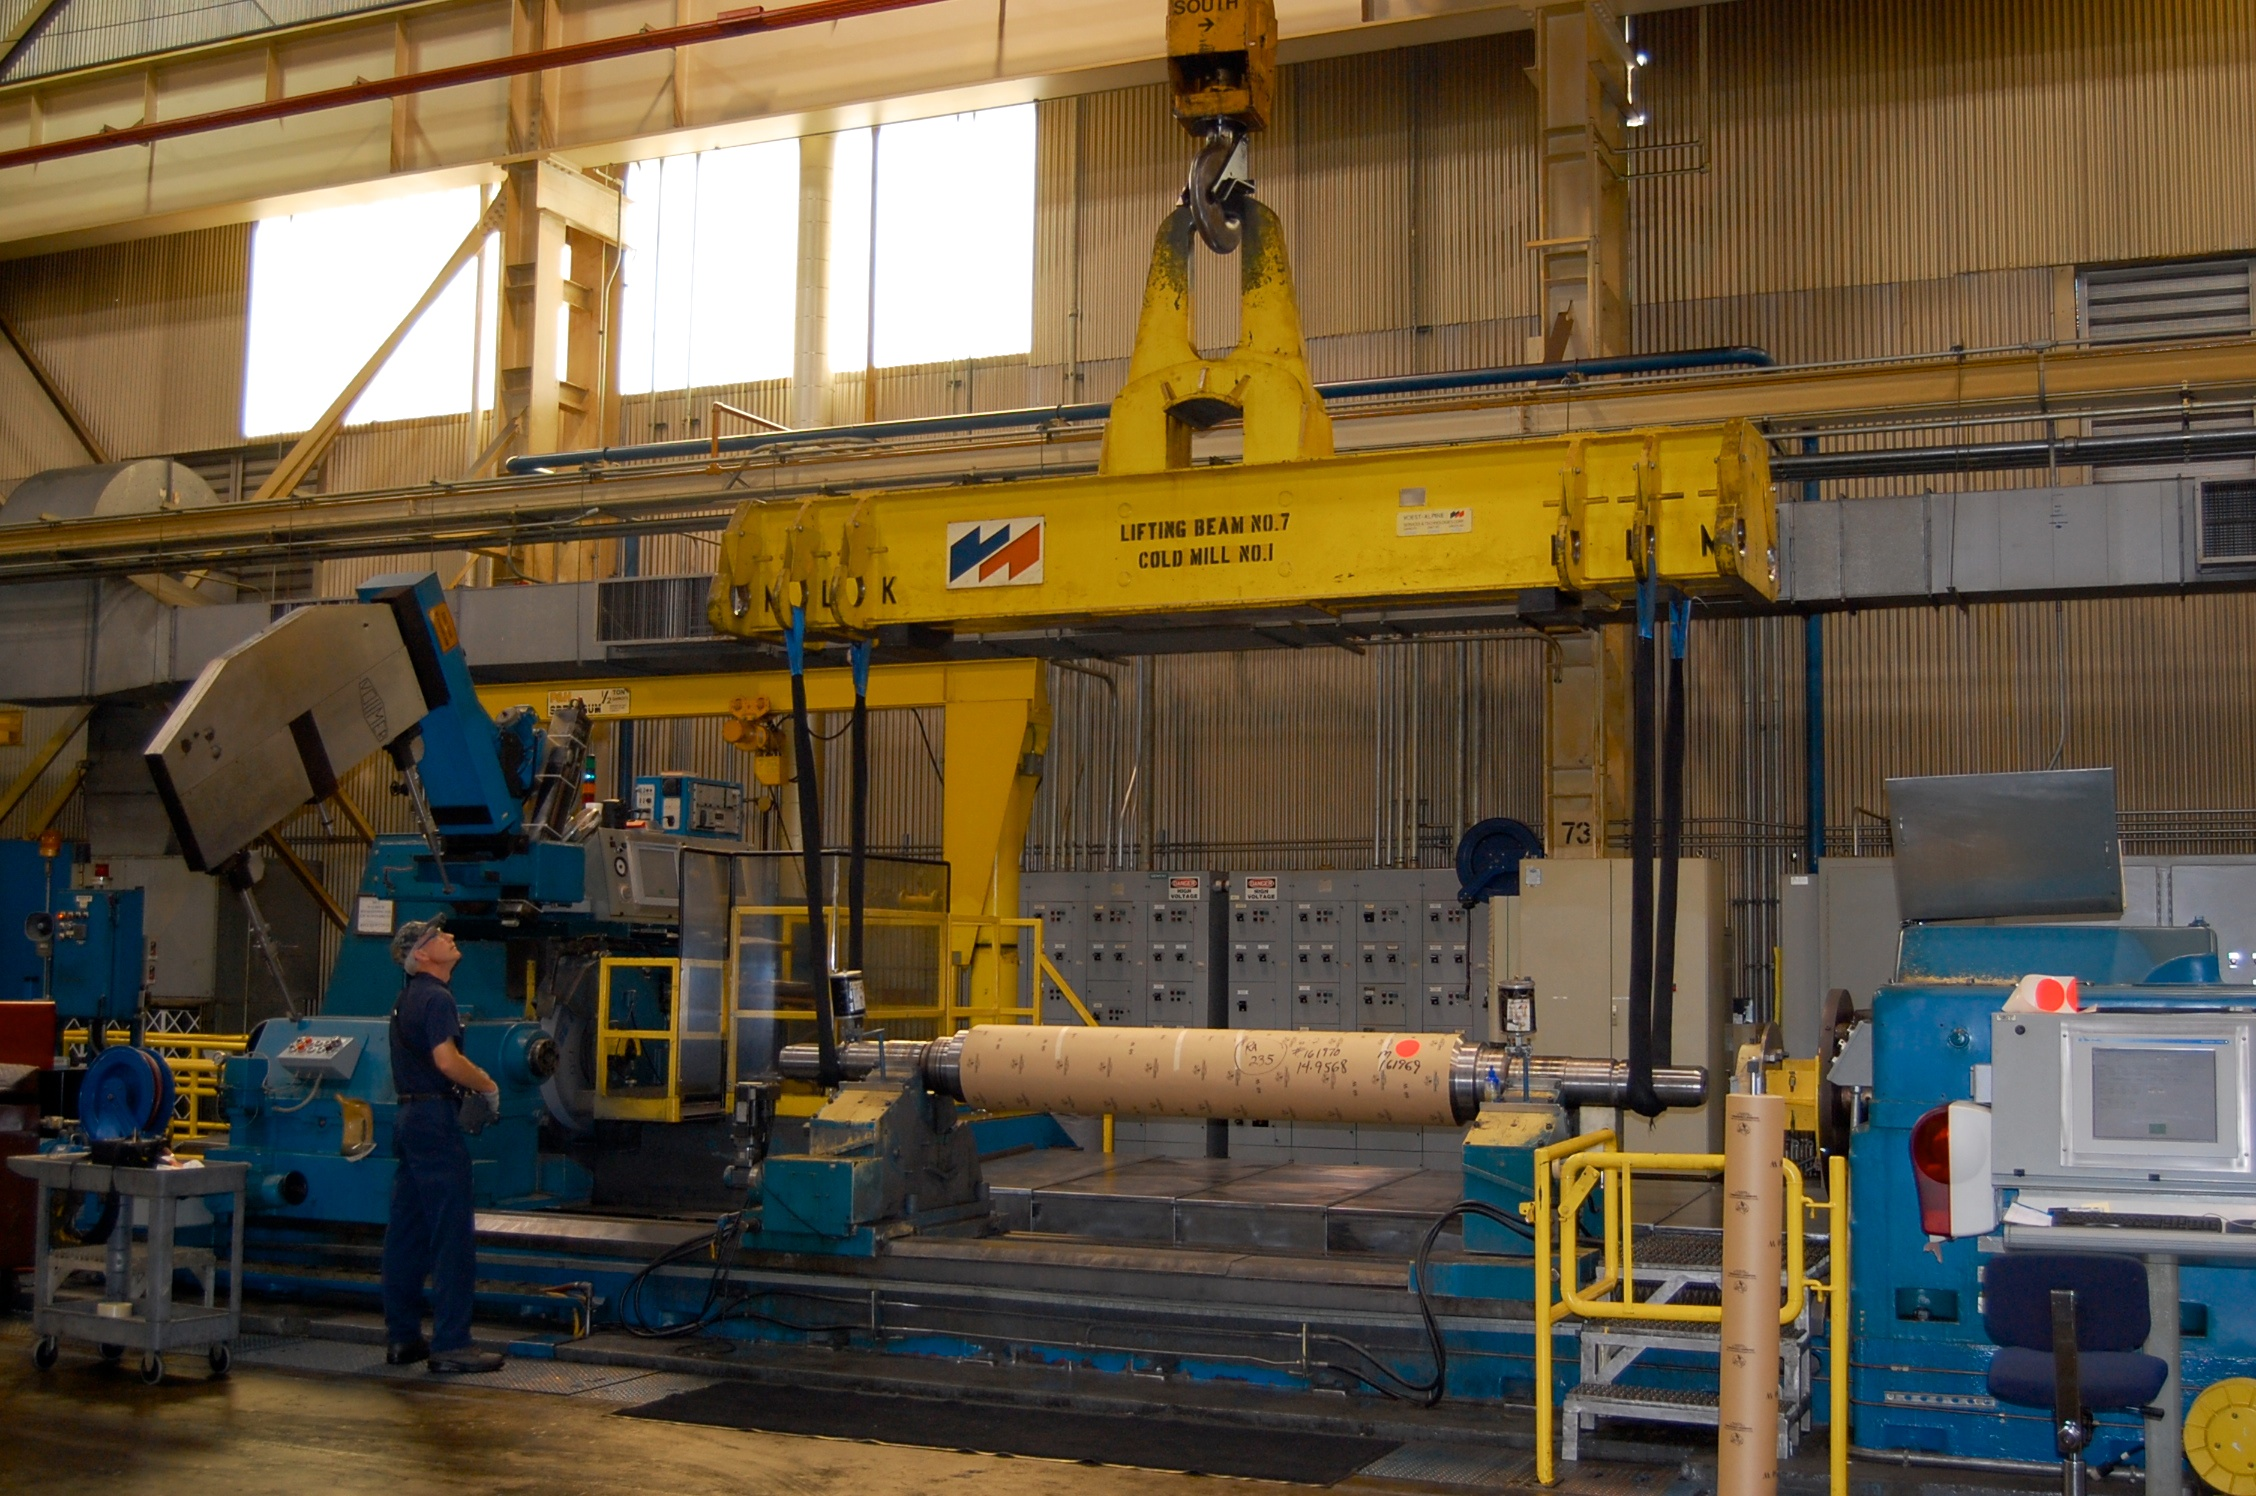
\includegraphics[width=3.5in]{crane}
\caption{CRANE OPERATOR POSITIONING PAYLOAD}
\label{CRANE OPERATOR POSITIONING PAYLOAD}
\end{center}
\end{figure}

In overhead cranes, the payload is suspended from a trolley that moves along the bridge. The bridge itself can also move, so that the crane can serve a large area. Figure 1 shows a typical bridge crane. Accidents in overhead crane operation remain a problem, causing damage and injuries\cite{beavers}. According to Crane Inspection and Certification Bureau, 90\% of all crane accidents occur due to human error\cite{cicb}. Half of U.S. crane accidents that had injuries in 2009 resulted in fatalities.

Recent developments in crane vibration reduction research have greatly reduced the vibration of the crane, improving safety and efficiency. One of these techniques is input shaping\cite{Smith},\cite{Seering},\cite{w.sing}. It shapes the command input by convolving a sequence of impulses with crane operator input. The convolved signal is then used as the reference command. This technique has proven useful for vibration reduction of cranes\cite{Singer},\cite{Sorensen},\cite{Khalid},\cite{Kim}.

Control techniques like input shaping reduce the probability of crane collisions with obstacles. However, lack of knowledge of the workspace and common limitations in human perception of distance and depth still limit the ability of the operator to safely move a crane through a workspace. One possible solution to these limitations is aiding the operator with a map of the workspace that depicts the current position of obstacles. The map could be extended to include information about past locations of obstacles as well. The past locations could be an indication of the possibility of finding an obstacle at a given location in the workspace.

Research has been conducted to model the workspace in order to avoid crushing obstacles during operations of heavy equipment\cite{changwan}.
Vision systems have been used for mapping and navigation for mobile robots\cite{murray},\cite{felix},\cite{stiller} and developing augmented reality workspaces\cite{klein},\cite{km}. Simultaneous Localization and Mapping (SLAM) is a well established method for mapping an unknown environment, or updating a map within a known environment by mobile robots and autonomous vehicles while at the same time keeping track of their current locations\cite{sebastian},\cite{dissa}.

 A machine vision system has been implemented on tower cranes\cite{Aviad},\cite{Yang}. The sole purpose was to help the operator see the workspace clearly. Some researchers have used machine vision as a means of measuring the crane hook location for feedback control\cite{Yoshida:06}. However, there was no attempt to map the crane workspace.
This paper describes a novel approach of mapping the crane workspace in near-realtime using machine vision.

In the following sections, the object detection and mapping techniques are explained. First, the steps of image processing, background detection, obstacle detection, elimination of payload from map and stitching technique are discussed. Next, a method for combining current and older images to produce the final map is described. Then, the effect of changing the design parameters on the mapping performance is explained. Finally, the conclusions made from this research are discussed.

%%%%%%%%%%%%%%%%%%%%%%%%%%%%%%%%%%%%%%%%%%%%%%%%%%%%%%%%%%%%%%%%%%%%%%
\section*{Overview of Mapping}


\begin{figure}[tb]
\begin{center}
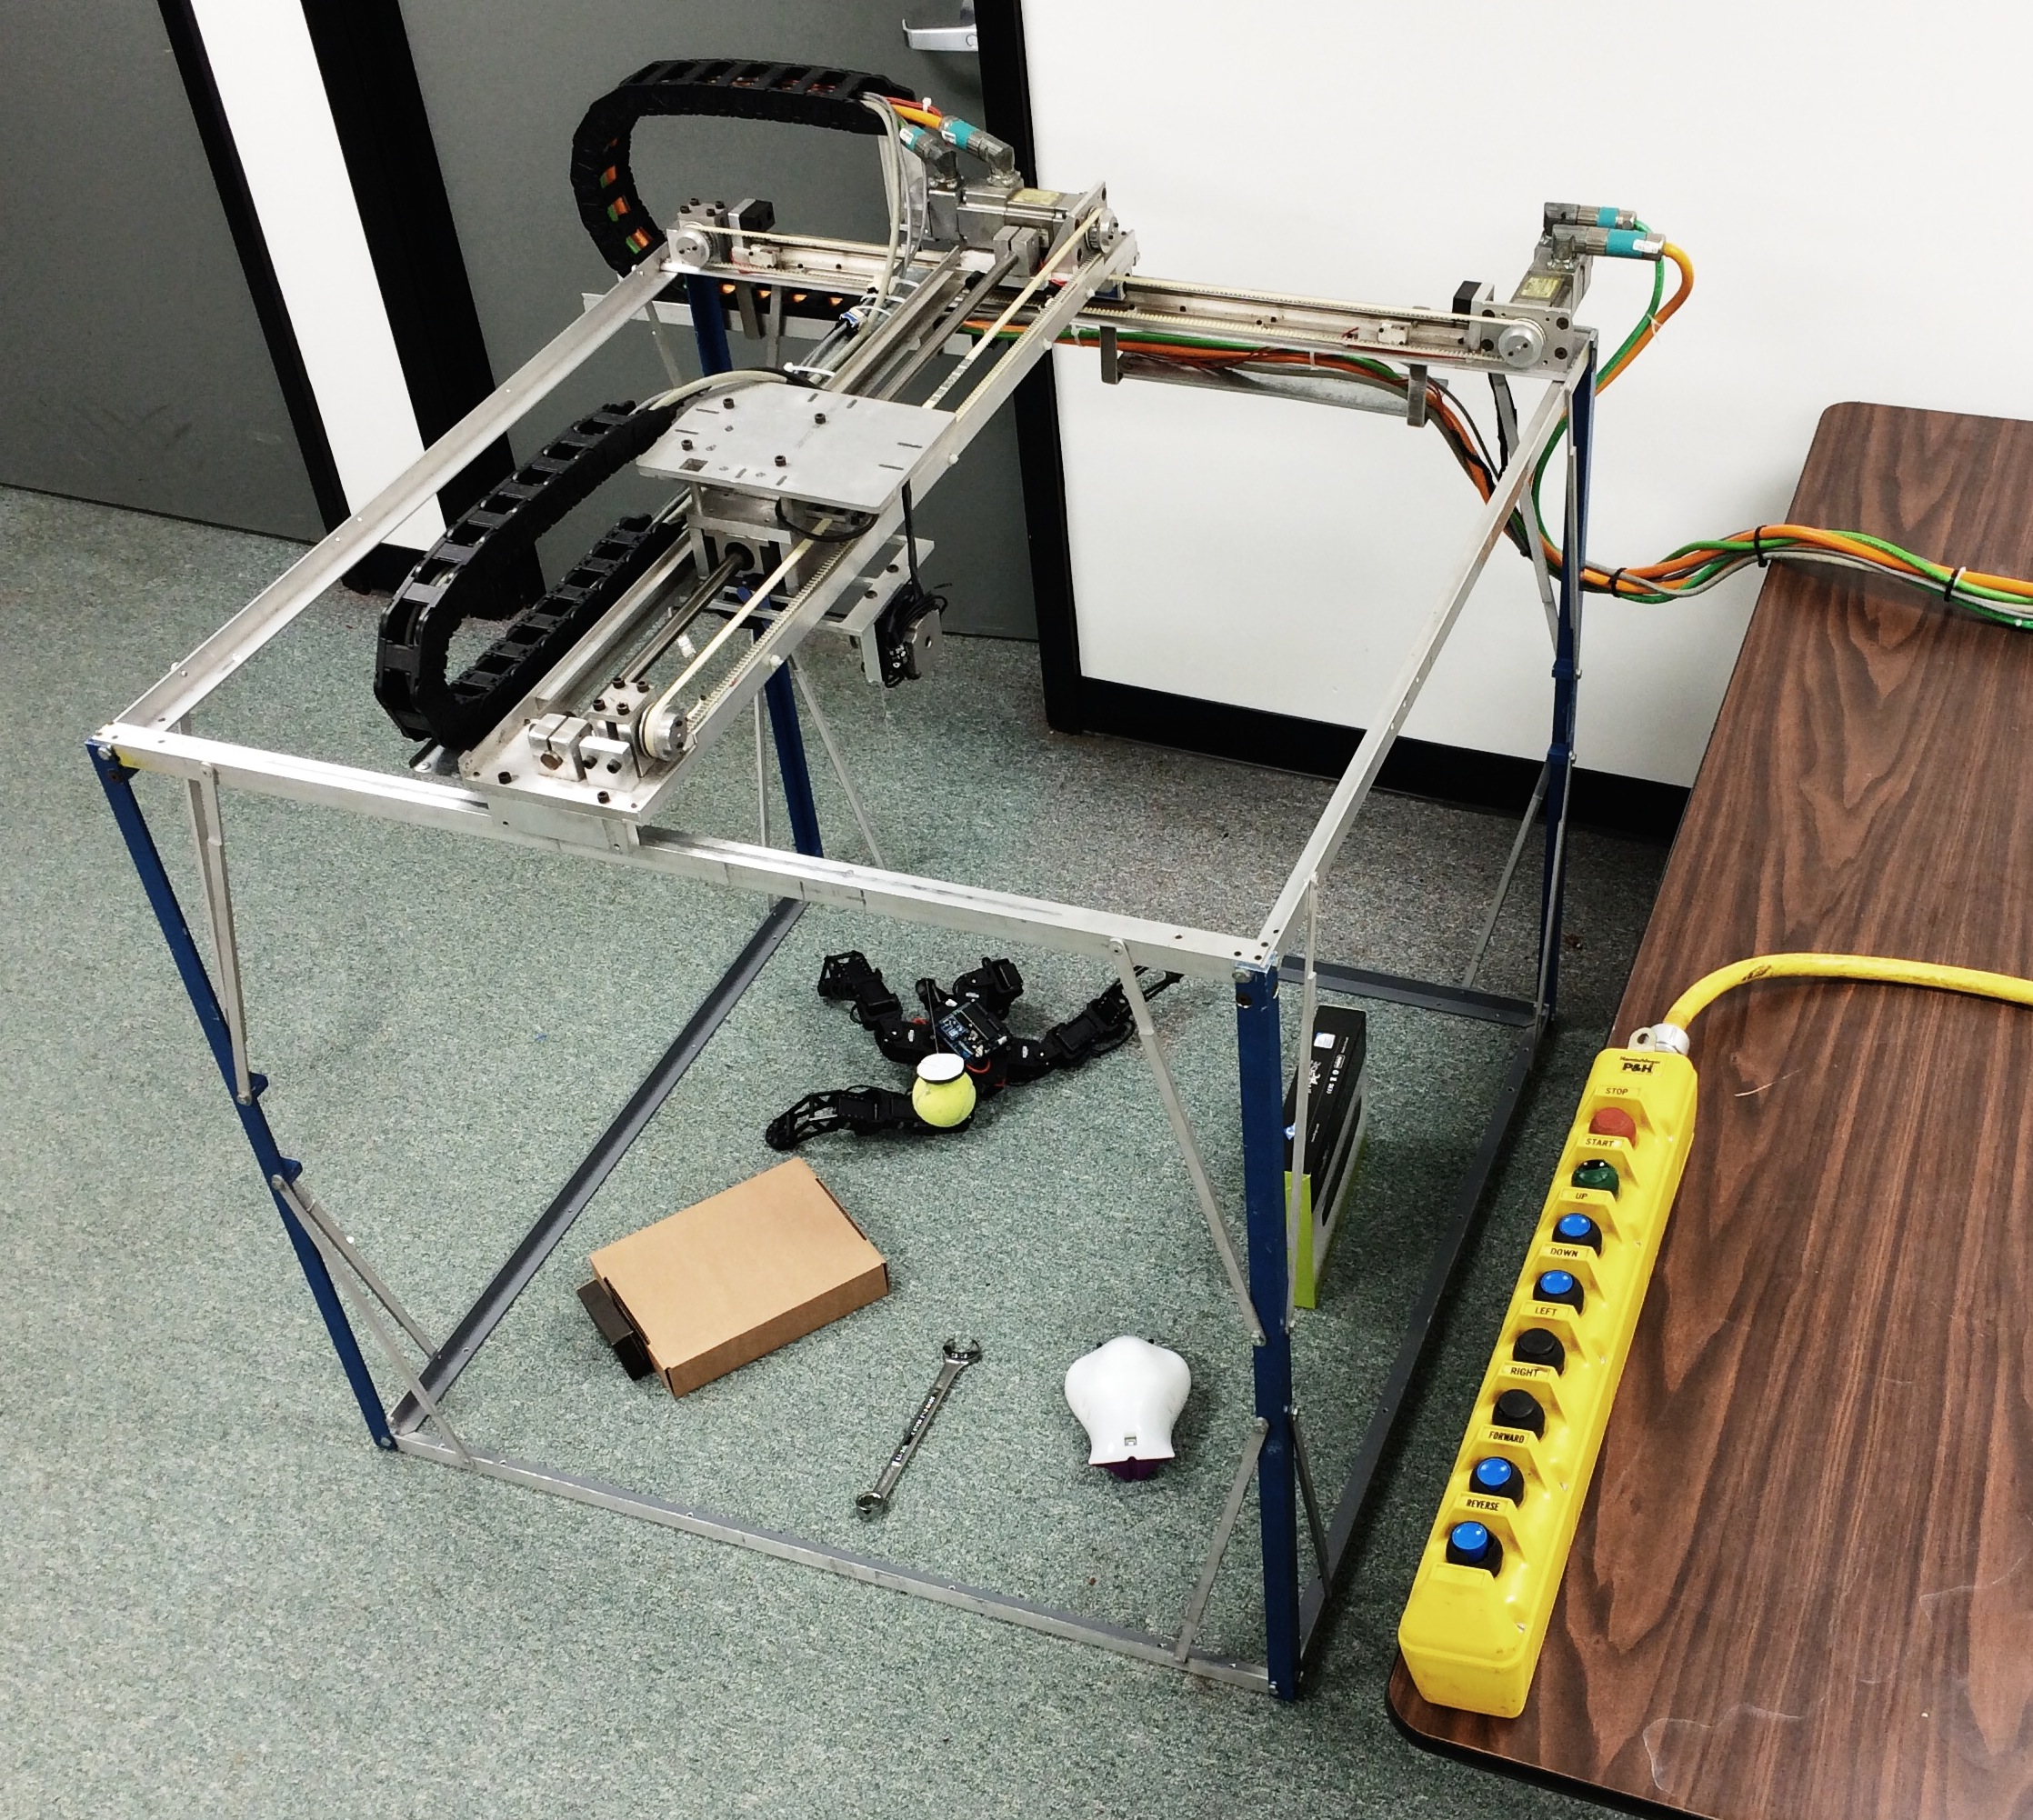
\includegraphics[width=3.5in]{scale_crane}
\caption{SCALE CRANE USED FOR THE EXAMPLES IN THIS PAPER}
\label{default}
\end{center}
\end{figure}

\begin{figure}[t]
\begin{center}
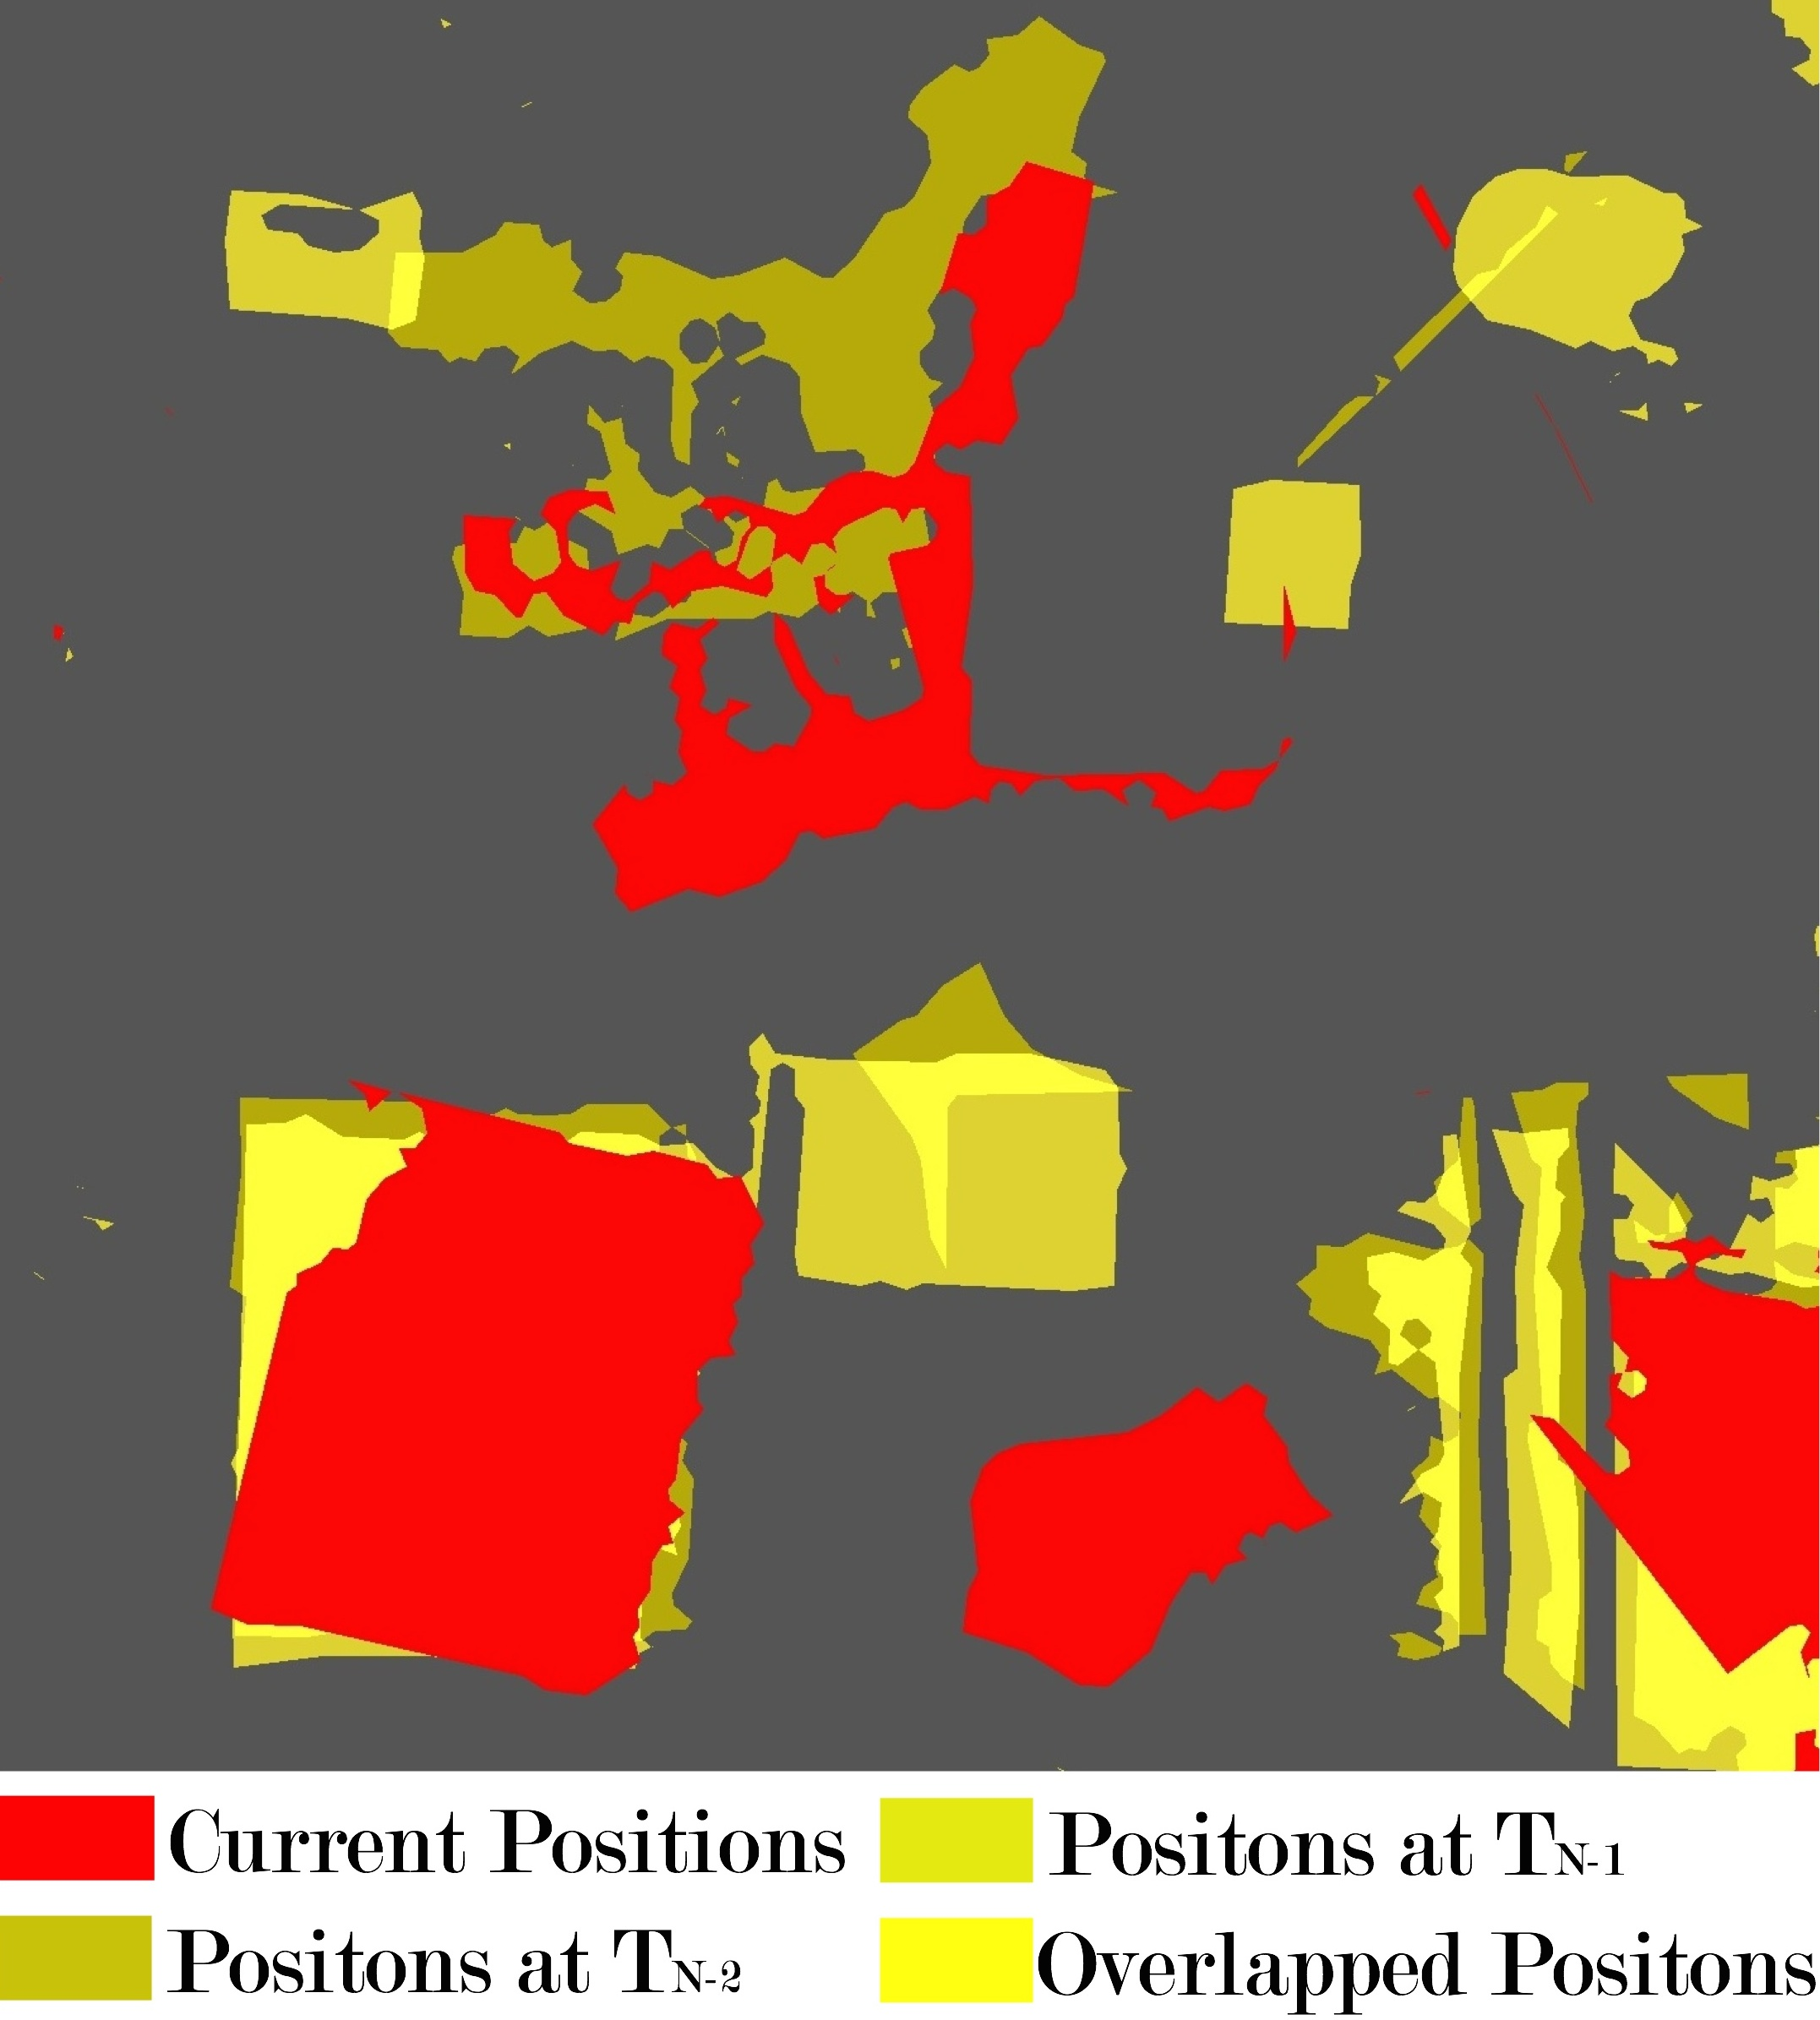
\includegraphics[width=3.5in]{overlapped}
\caption{CRANE WORKSPACE MAP}
\label{default}
\end{center}
\end{figure}

\begin{figure}[htbp]
\begin{center}
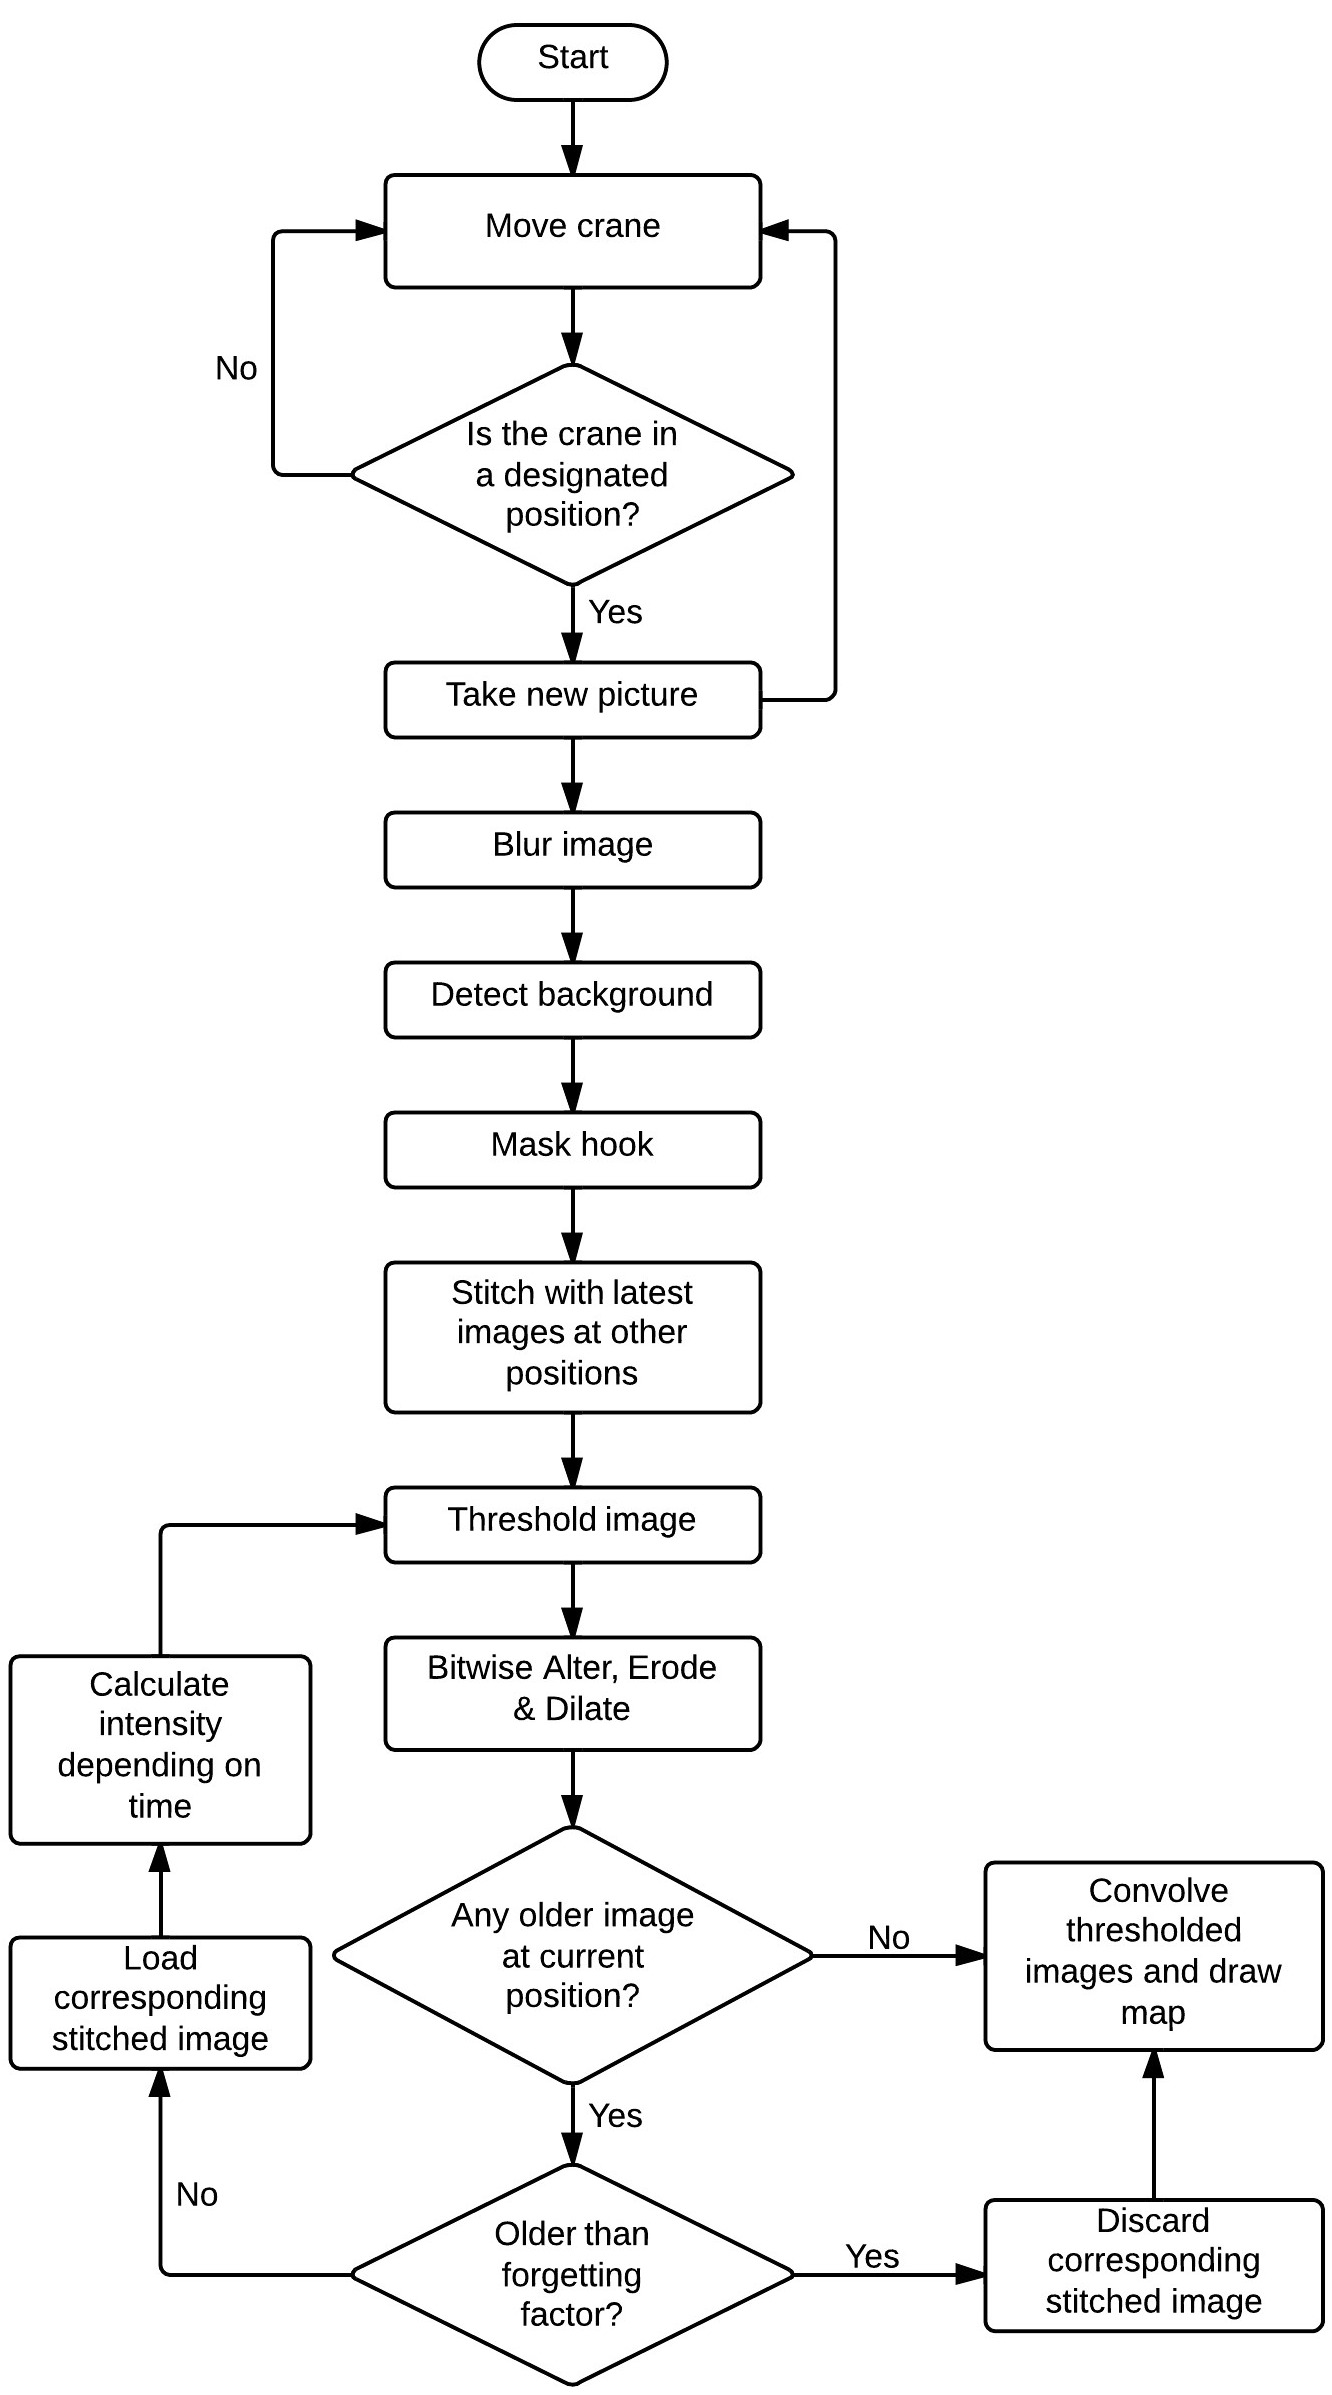
\includegraphics[width=3.5in]{crane_flowchart}
\caption{FLOWCHART OF THE MAPPING PROCESS}
\label{default}
\end{center}
\end{figure}

Figure 2 shows the crane used for the examples presented in this paper. The workspace of this crane is 1m x 1m x 1m. It is controlled using a Siemens PLC and is driven by Siemens AC servomotors.

For the mapping technique presented in this paper, a camera is mounted on the crane trolley. The camera automatically takes a picture at predefined points in the workspace. These images are then processed. The background is detected, and the crane hook is masked. Then, the obstacles are identified and a graphical representation of the workspace is generated. 

%The position and time information of each image is used to show zones where the possibility of finding obstacles is greater,  based on past obstacle locations. 

An example map resulting from this process is shown in Figure 3. The map presented in this paper shows the current locations of the obstacles in red and past obstacle locations in yellow. The intensity of the yellow regions indicate how recently an obstacle was found at that location. For example, a high intensity of yellow indicates that an obstacle was at that location recently. This suggests that there is a higher probability of finding an obstacle there.

%The brightness of the yellow regions depends on how long ago there was an obstacle in that location, or how much overlap there is among obstacles at the same position at different times, if there is any. 

Figure 4 shows a flowchart of the entire process, each part of which is described in detail in the following sections.

%%%%%%%%%%%%%%%%%%%%%%%%%%%%%%%%%%%%%%%%%%%%%%%%%%%%%%%%%%%%%%%%%%%%%%
\section*{Individual Image Processing}
%For the mapping , OpenCV has been used with C++ as the programming language.OpenCV is a free online computer vision library .

In order to eliminate noise in the images, it is necessary to smooth the images first. Gaussian blur and median blur are two of the most commonly used methods for blurring. They are also used in this work. 
%\begin{figure}[htbp]
%\begin{center}
%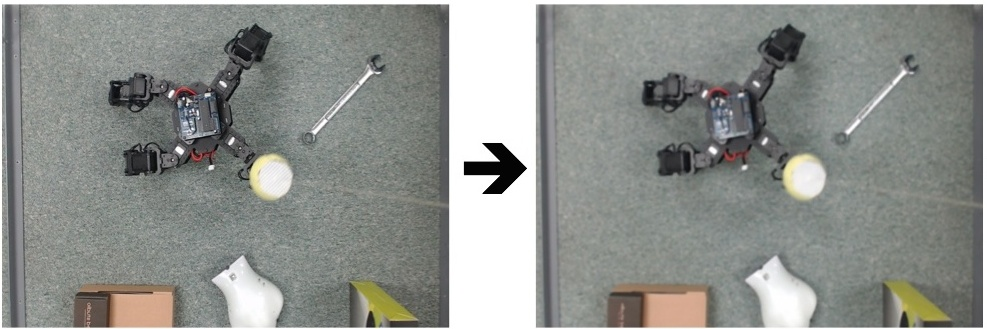
\includegraphics[width=3.0in]{blurred}
%\caption{IMAGE BLURRED}
%\label{default}
%\end{center}
%\end{figure}

To separate the obstacles from the background, it is necessary to detect the background. If the background is known, a simple thresholding can be used to separate the background from the foreground. However, depending on the noise level and lighting, the background may vary significantly. Moreover, the reflections of the lighting source and the shadows of the objects can make it difficult to distinguish the obstacles from the background. 

 For the method used in this research, each of the three channels of the image is divided into ranges of equal length. Then, the pixels are scanned in each channel and the number of pixels that fall into each range are counted. The range where most of the pixels fall into is the background value range of that image in that channel; it is assumed in this work that the background occupies larger area than obstacles. In most cases, the background pixel values have significant variation. Instead of scanning each pixel, a number of pixels are skipped while scanning to get the correct background. Skipping pixel also saves computation power. The optimum number of pixels to be skipped depends on the lighting conditions and noise level of the workspace. The effect of number of pixels skipped on obstacle detection is discussed later.

%Scanning every pixel takes a big portion of computing power. One solution is skipping pixels. It eliminates the possibility of highly concentrated small areas to be considered as background. But how many pixels should be skipped remains a problem, because it is highly dependent on the noise level and lighting condition of the workspace. Good results came in experiment when every 700-1000 pixels were skipped.

Because the camera can not capture the entire workspace in a single image, the individual images need to be stitched together. However, there will always be the crane hook/payload in the image, because the camera is mounted directly over the the hook. A simple solution is to cover that part of image with the average background color calculated, as shown in Figure 5. The part of the workspace area blocked by the hook can be recovered from neighboring images after stitching. The recovered workspace area is greater for a larger overlap between neighboring images.

%How much information from the blind spot is recovered depends on the amount of overlap among the images. A larger overlap means greater portion of area blocked by the hook recovered.

\begin{figure}[tb]
\begin{center}
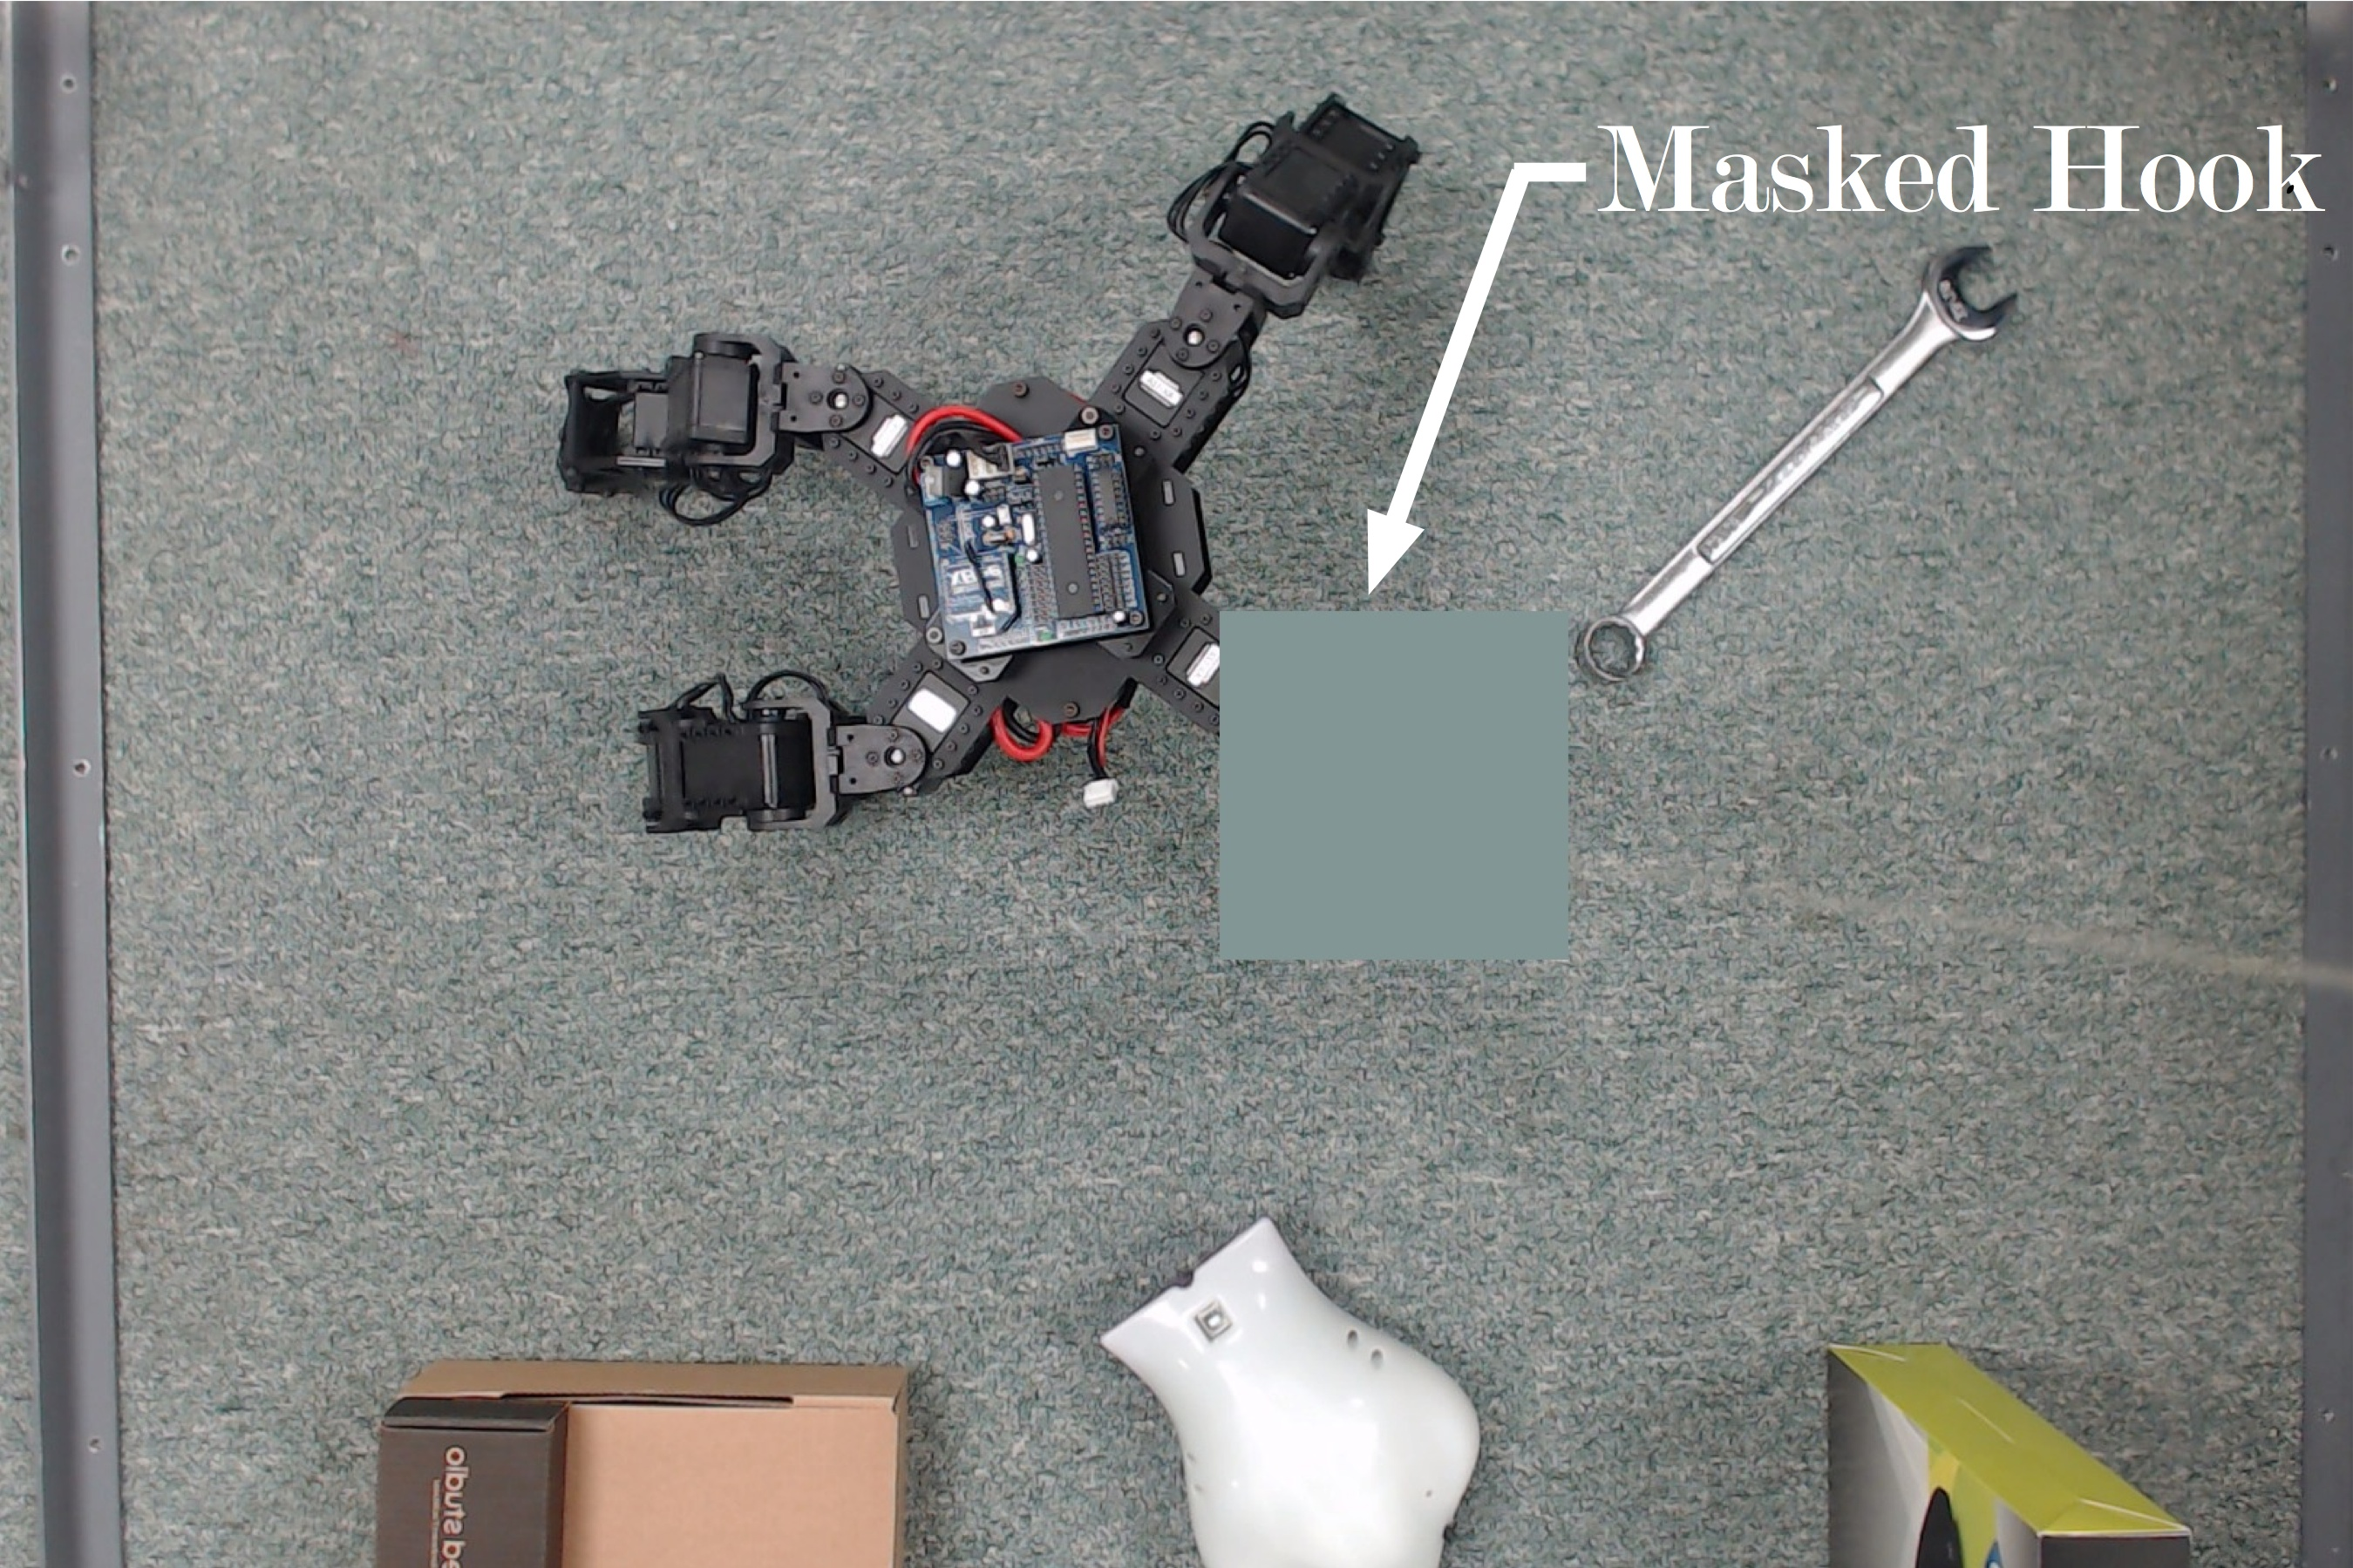
\includegraphics[width=3.5in]{masked}
\caption{CRANE HOOK MASKED}
\label{default}
\end{center}
\end{figure}

%Though it is assumed that input shaping is applied in the crane control system and the payload is always at the center of the image, a small sway of the payload makes it difficult to mask it. It is necessary to know the precise position of the payload to completely mask it.
%OpenCv stitcher class is used to stitch the images together. It consumes a significant amount of memory. Using the graphical processing unit for stitching significantly reduces the stitching time. 
After masking, the images are stitched together as shown in Figures 6 and 7. In order to stitch images, the key-points among them are matched. The larger the overlap between neighboring images is, the more key-point matches are found, yielding a better stitching performance. However, greater overlap means more individual images are required to cover the workspace. This takes more time and computation power to stitch.
%This is so because in order to stitch the OpenCv stitcher class detects key points in both images and tries to match them. Plane Warper should be selected to warp the images.

\begin{figure}[t]
\begin{center}
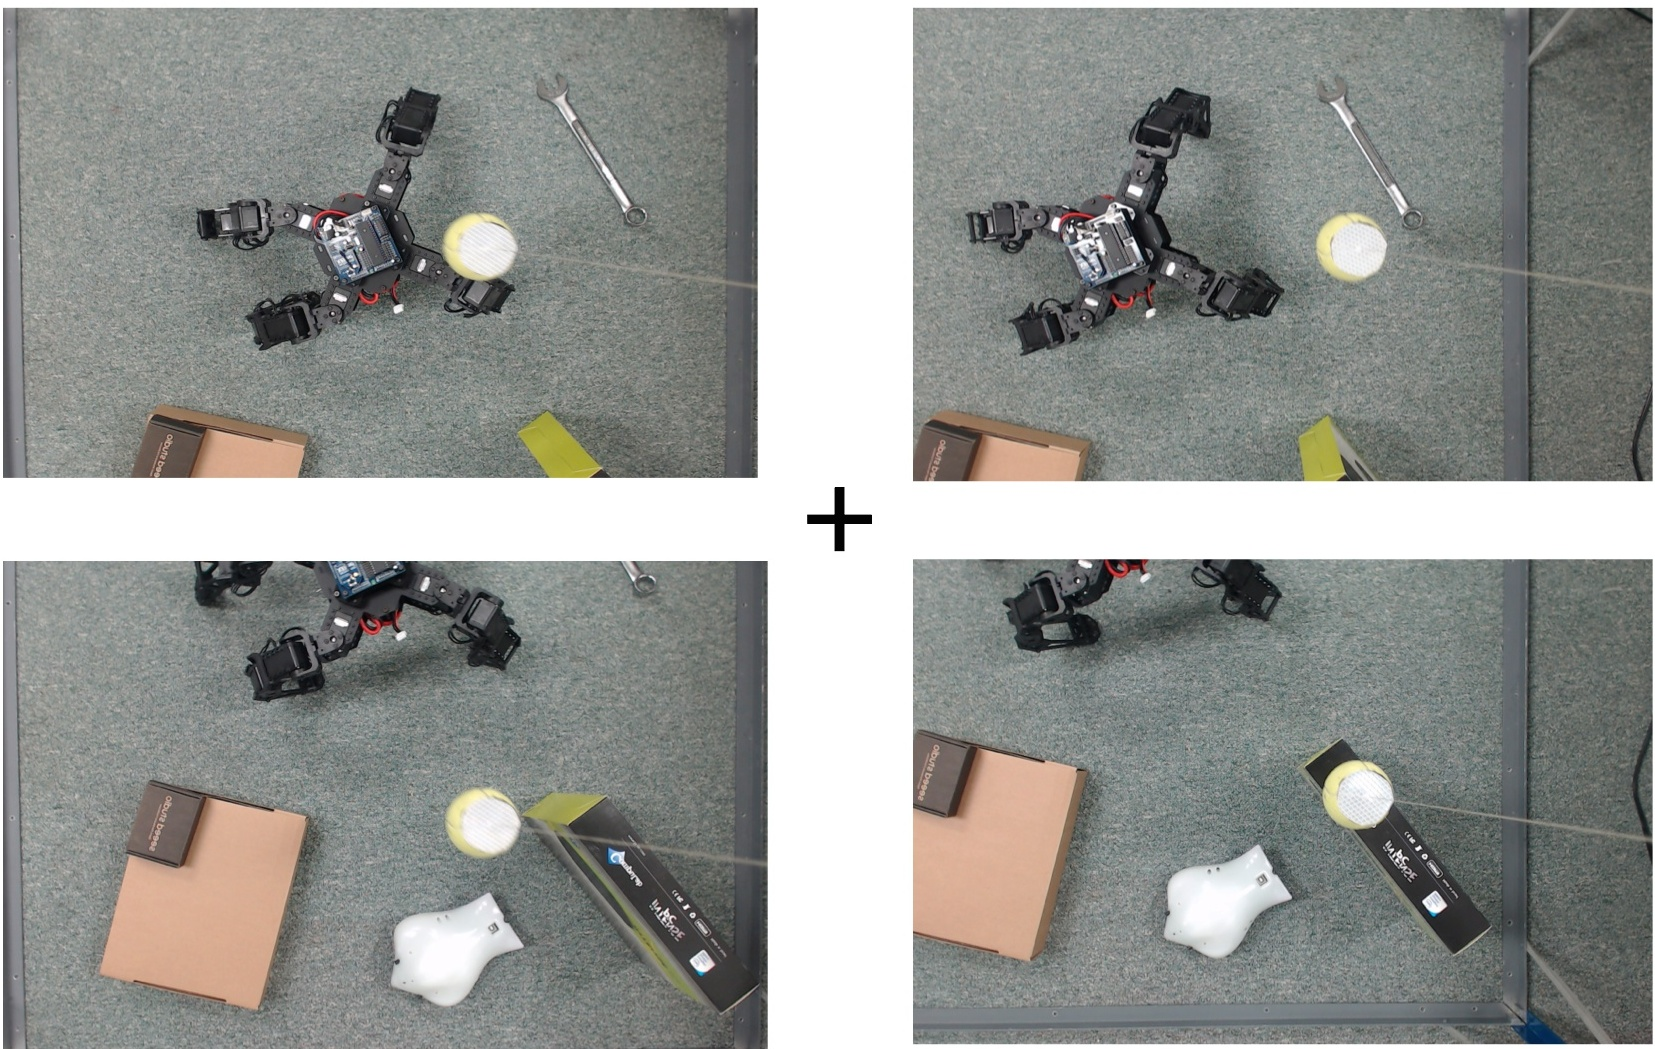
\includegraphics[width=3.5in]{individual}
\caption{INDIVIDUAL IMAGES}
\label{default}
\end{center}
\end{figure}


\begin{figure}[t]
\begin{center}
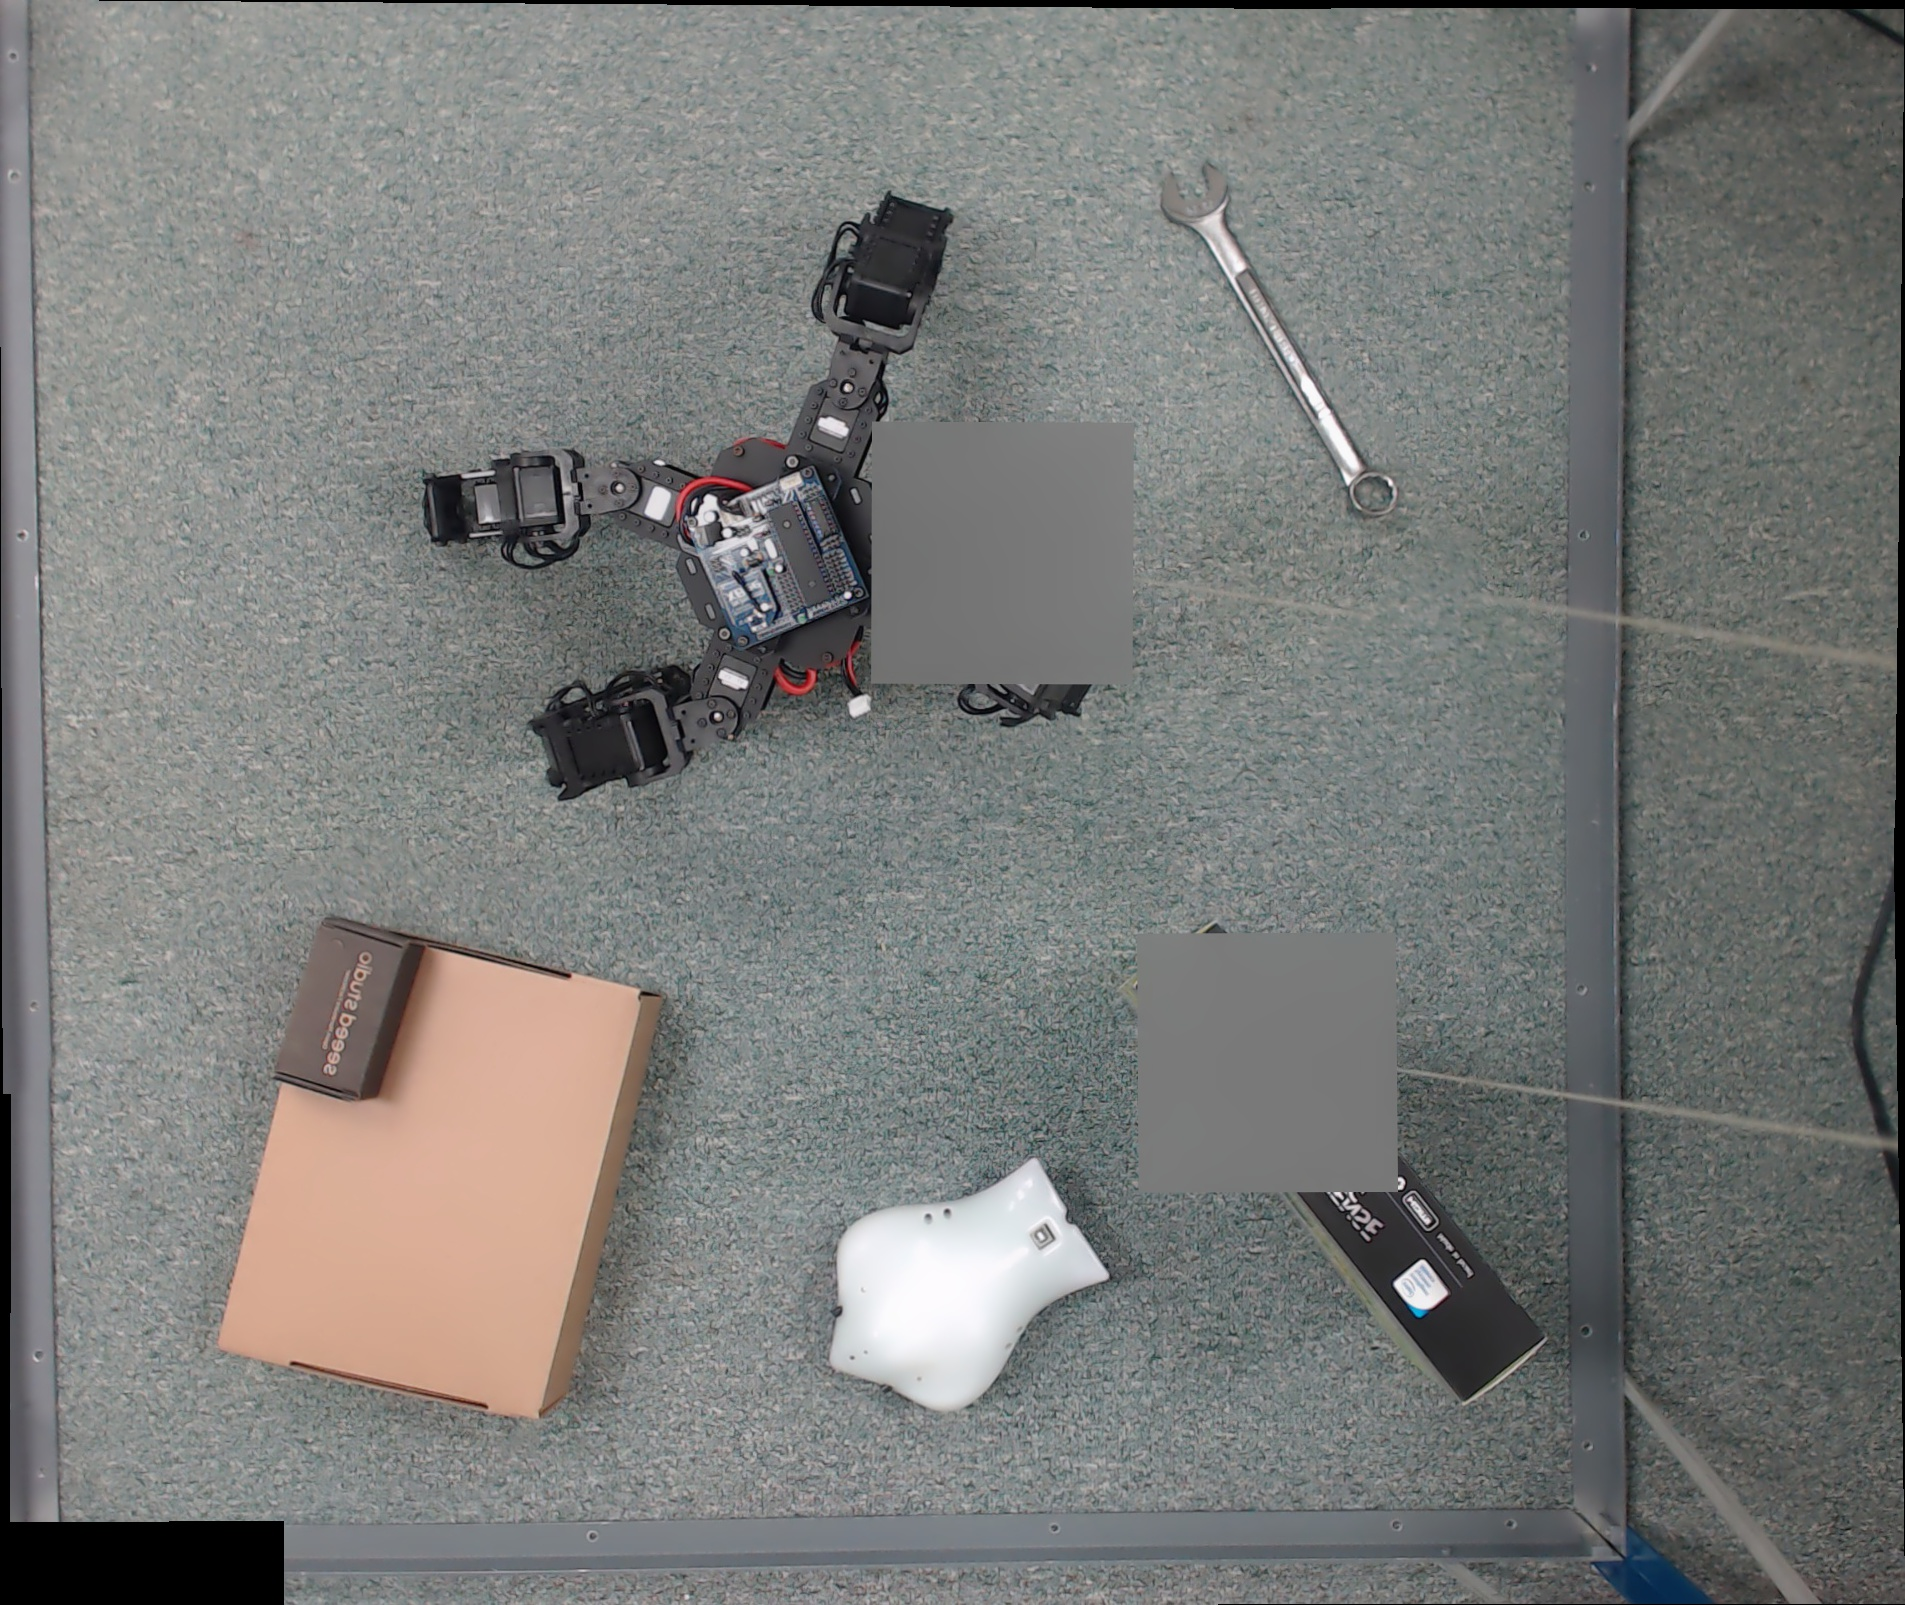
\includegraphics[width=3.5in]{stitched}
\caption{STITCHED IMAGE}
\label{default}
\end{center}
\end{figure}

Next, all three channels of the stitched image are thresholded simultaneously through two three-channel scalars close to the background color. The range of these scalars depends on the degree of noise in the background. For example, a small threshold is sufficient for a low-noise and clear background, and gives clean image after thresholding, where every obstacle is perfectly detected. The resultant image after thresholding is a binary image, which should be bitwise altered and  further refined using erosion and dilation to get rid of small blobs. Figure 8 shows thresholded and bitwise altered images, and Figure 9 shows dilated and eroded images.
 
% the background being 1 and all other objects 0. %Using bitwise_not function reverses them.

%To refine the image we have, we use erosion and dilat functions.These two functions removes the unwanted small blobs from the thresholded image.

\begin{figure}[t]
\begin{center}
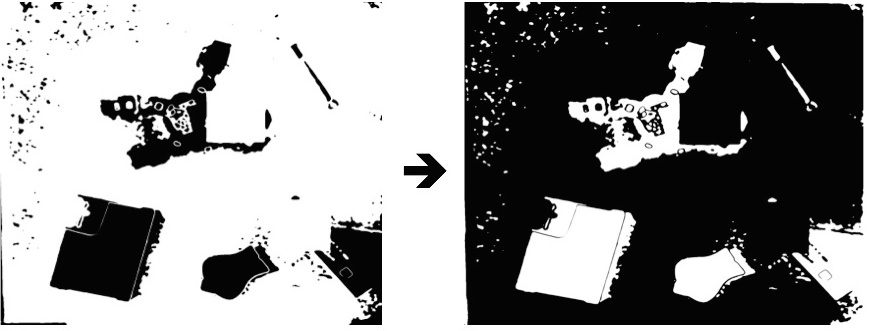
\includegraphics[width=3.5in]{thresholded}
\caption{THRESHOLDED AND ALTERED IMAGE}
\label{default}
\end{center}
\end{figure}

\begin{figure}[t]
\begin{center}
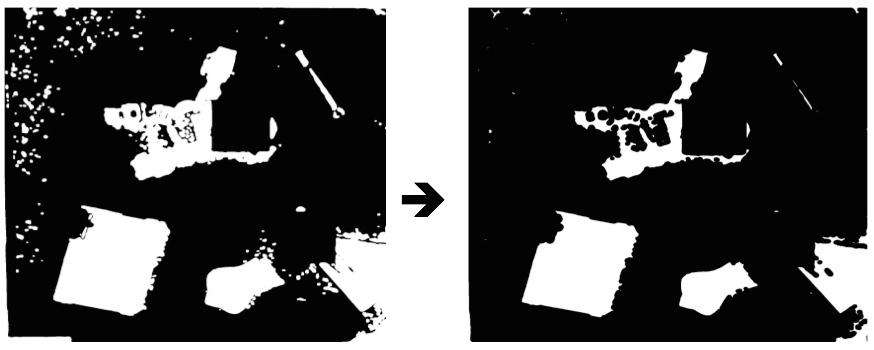
\includegraphics[width=3.5in]{dilated}
\caption{DILATED AND ERODED IMAGE}
\label{default}
\end{center}
\end{figure}


After erosion and dilation, the contours of the obstacles are extracted. Then, a polygonal curve is estimated using the Douglas-Peucker algorithm, and the contours are drawn, as shown in Figure 10. 

%The color used to draw the contours is a linear/exponential function of time when the images are taken, to make it apparent how long ago there was an obstacle in that place and if there is any right now. If the color is red, it shows the positions of the obstacles found from latest images. Brighter shades of yellow show recent positions of the obstacles while darker shades show older.

\begin{figure}[t]
\begin{center}
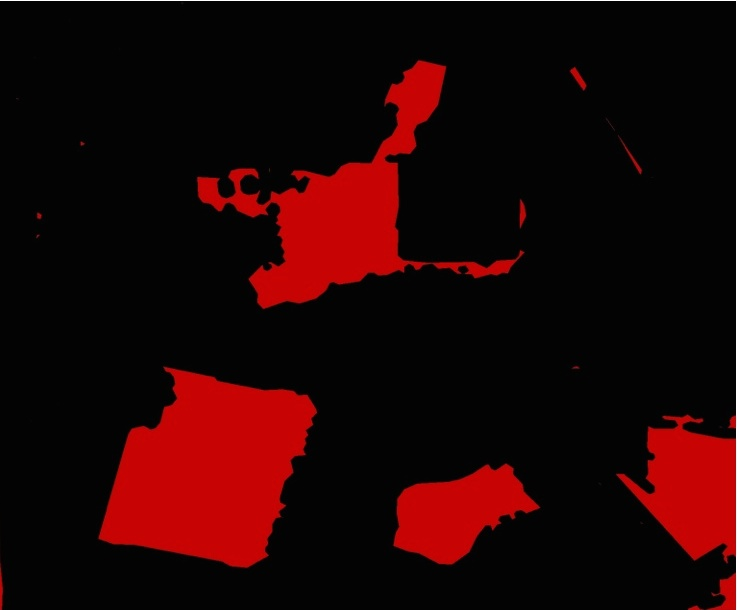
\includegraphics[width=3.5in]{contour}
\caption{IMAGE AFTER CONTOUR IS DRAWN}
\label{default}
\end{center}
\end{figure}


\section*{Mapping}
The mapping process presented in this paper takes the latest, as well as older positions, of the obstacles into account. The older positions of obstacles can be used as an indicator of the likelihood of there being an obstacle at that location in the future.
% If an obstacle appears just once in a position, then it might be just a moving object or human being. This areas are not considered as high-risk areas unless obstacles are detected in most recent images.

Each time a new picture is taken by the camera at a particular position, an individual map is generated by stitching that picture with the most recent pictures at other positions. Then, a final map is created by convolving the latest map with older individual maps. 

%In the final map, the latest positions of the obstacles are shown in red to indicate certainty of finding an obstacle, and all other positions in yellow to show probability of finding an obstacle. The probability is indicated by the intensity of yellow. 

The individual maps are convolved in a way that the latest map is shown in red to indicate certainty of finding an obstacle. Older maps are shown in yellow, the intensity of which decreases linearly with time when that maps were generated. Relatively recent maps are more likely than older maps to indicate an obstacle position. The intensity decreases with time to show the decreased probability of finding an obstacle at that location. The slope of linearity determines how fast the individual maps lose weight as they get older.

Using multiple older images at a given location provides additional information. If there is an overlap in the yellow regions from past images, the overlapped area is brighter than in the individual maps. The overlapped area indicates there has been an obstacle present at these overlapping locations in the workspace at multiple times. This suggests that the probability of finding an obstacle there in the future is greater.

If an individual map is too old, it is forgotten. A memory factor determines when an individual map is forgotten. The bigger the memory factor is, the older an individual map can be and still taken into account for generating the final map.
% The recent obstacle positions are shown in bright yellow, and the older obstacle positions are shown in dark yellow. The color intensity represents how frequently or how recently the obstacles appeared in a particular position, hence the probability of finding an obstacle. The latest positions are always shown in red to indicate the certainty of finding an obstacle. 
%The crane can be programmed to never enter the red areas, and slowing down at the yellow areas.

%In this research, the time when a particular image was taken determines its weight. The older the the image is, the less weight it gets, if it is older than a particular time, it is forgotten. The time when it is forgotten is called memory factor. Half-life can be used as memory factor.

%For overlapping the older image, a linear or exponential decay can be used. The weight of recent images reduce at a faster rate with time in case of exponential decay, but at a slower rate for older images. In case of linear decay, the weight of images reduce steadily as they get older. Images which are  too old can be discarded by choosing a memory factor. The choice of memory factor depends on how old an image is intended to be taken into consideration. For example, if half life is considered as memory factor, the images older than half life are discarded.

%The latest position of the obstacle is shown with a 100\% intensity of yellow. Then, the intensity of the older positions are calculated using time as variable. The greater the time is, the less weight the older images get, as calculated from the decay function, which could be linear or exponential. The half-life is also calculated. If the image taken is older than the half life, it is discarded. Finally, the images are convolved to create the final map. 
As an example, individual maps at times $T_{N}$, $T_{N-1}$, $T_{N-2}$  are shown in Figure 11, where N is number of images. The resulting map is shown in Figure 12. In the map presented here, the red areas show the most recent positions of the obstacles. Medium-bright yellow areas show next to the most recent positions, and the dark yellow areas show the oldest positions of the obstacles. The overlapping areas between the older obstacle positions are shown by the brightest shade of yellow.

\begin{figure}
        \centering
        \begin{subfigure}[b]{0.15\textwidth}
                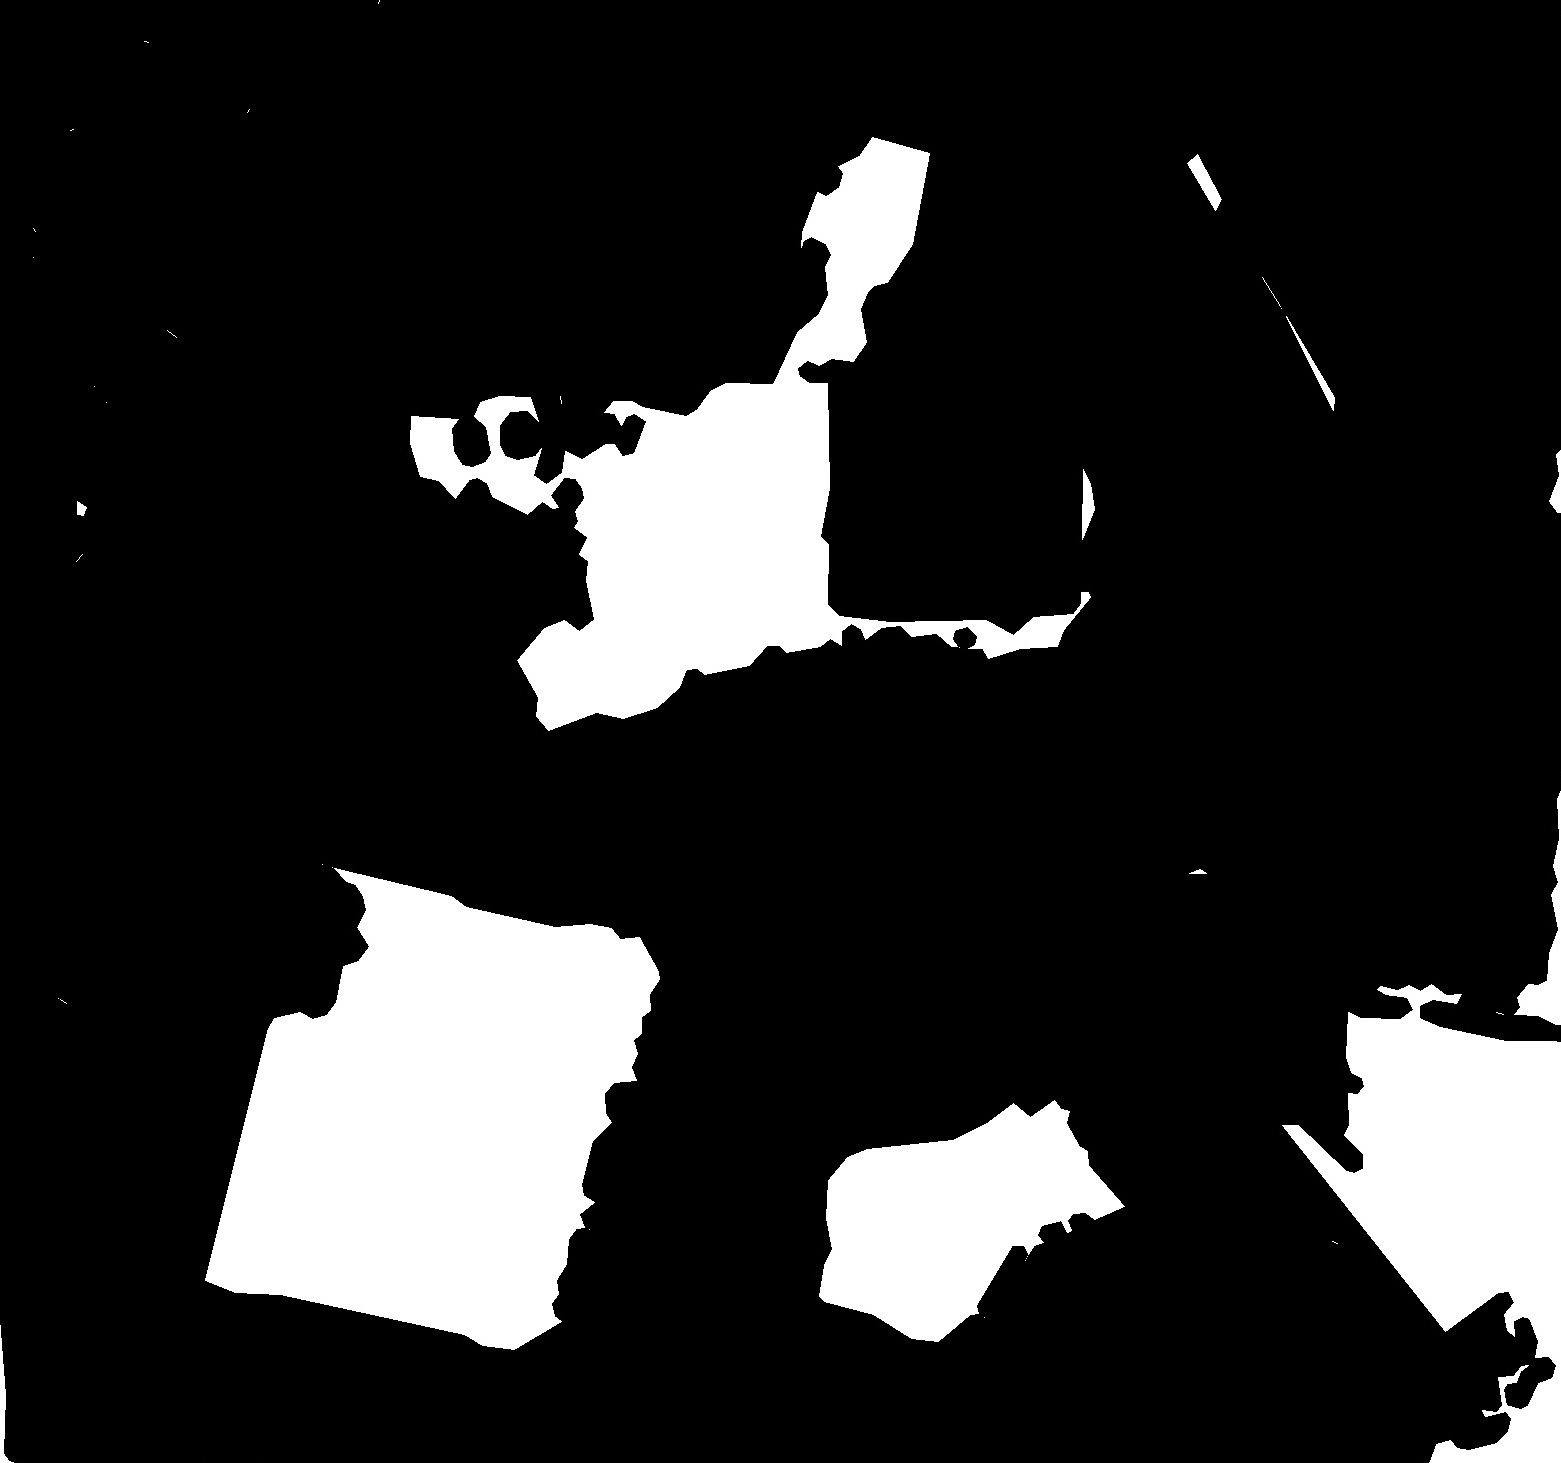
\includegraphics[width=\textwidth]{processed2}
                \caption{Time = $T_{N}$}
                \label{fig:latest image}
        \end{subfigure}%
        ~ %add desired spacing between images, e. g. ~, \quad, \qquad etc.
          %(or a blank line to force the subfigure onto a new line)
        \begin{subfigure}[b]{0.15\textwidth}
                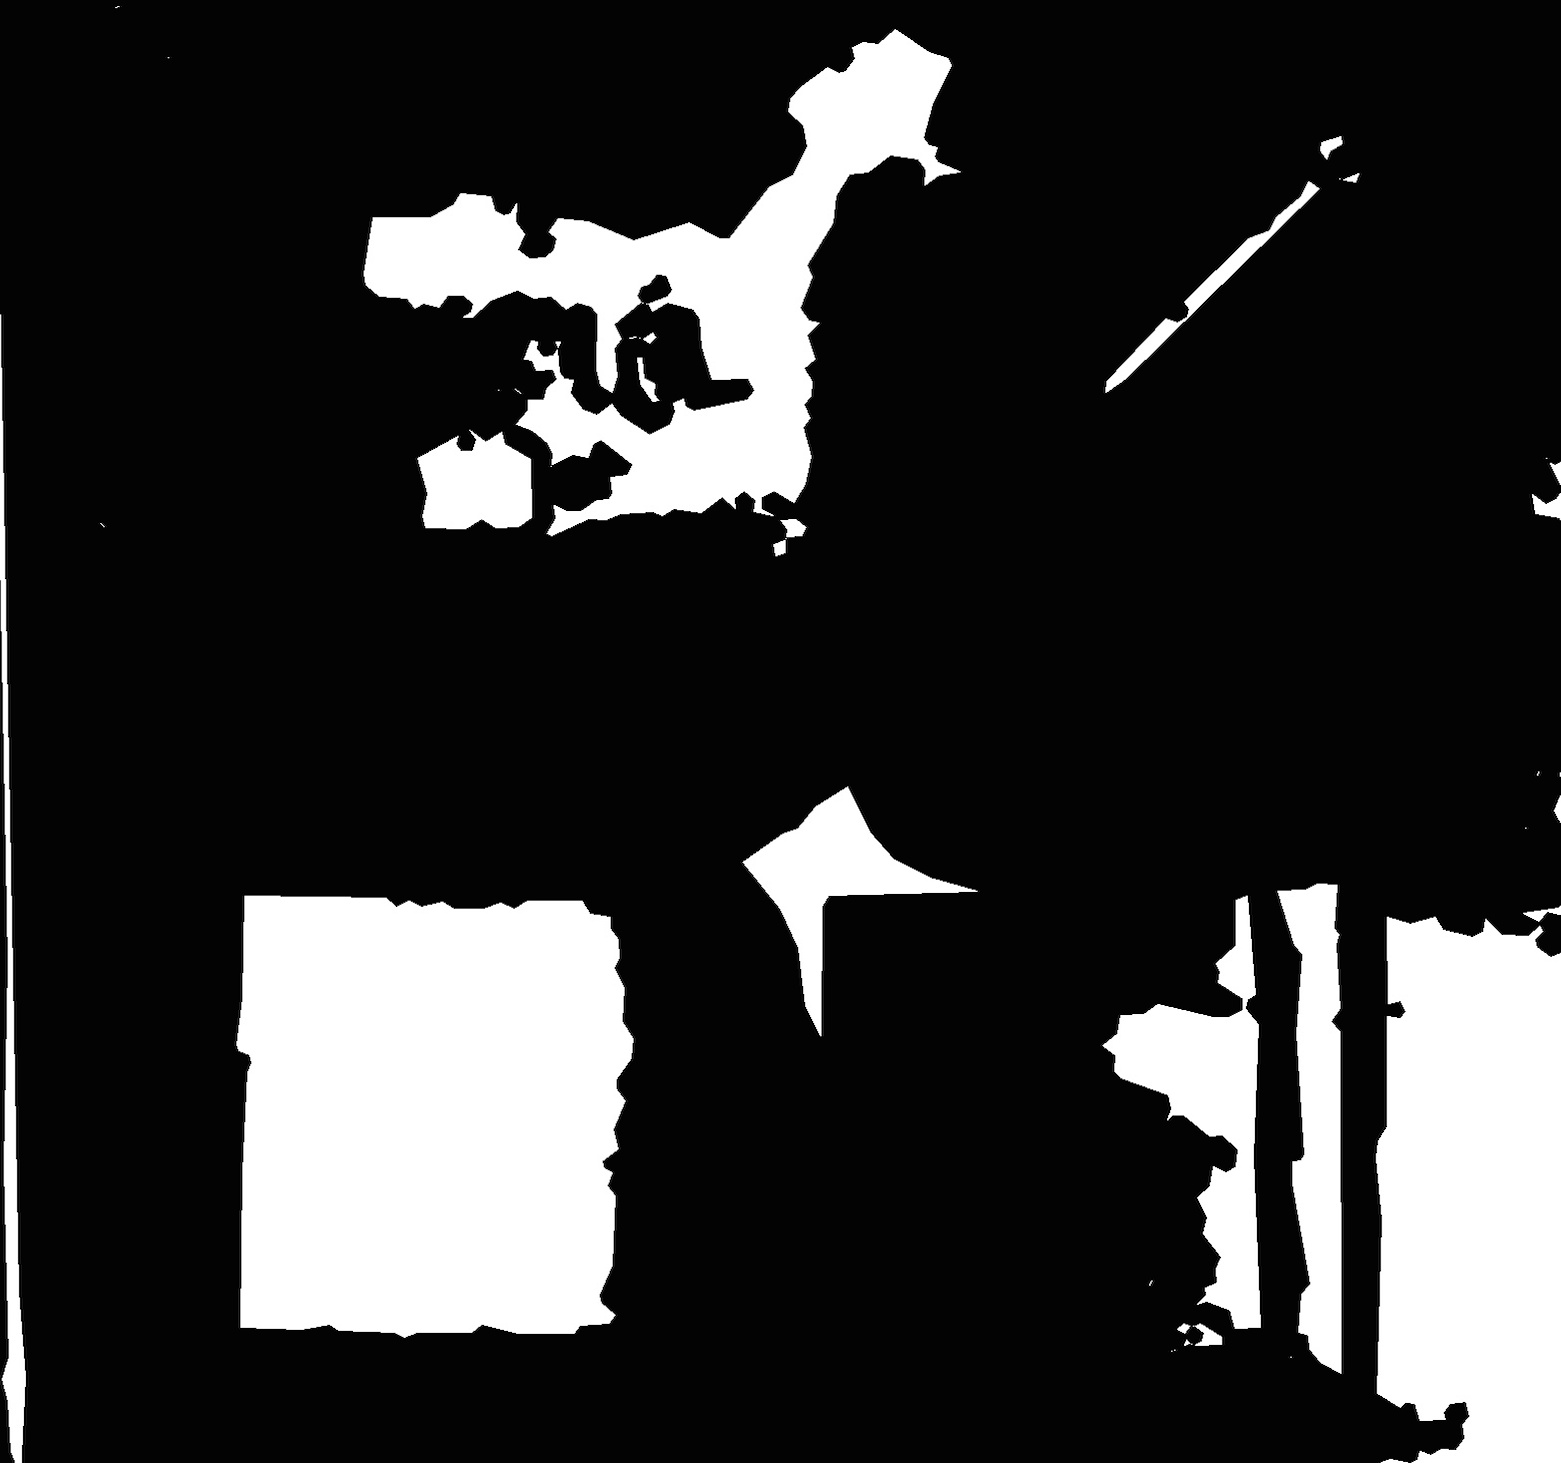
\includegraphics[width=\textwidth]{processed4}
                \caption{Time = $T_{N-1}$}
                \label{fig:second latest image}
        \end{subfigure}
        ~ %add desired spacing between images, e. g. ~, \quad, \qquad etc.
          %(or a blank line to force the subfigure onto a new line)
        \begin{subfigure}[b]{0.15\textwidth}
                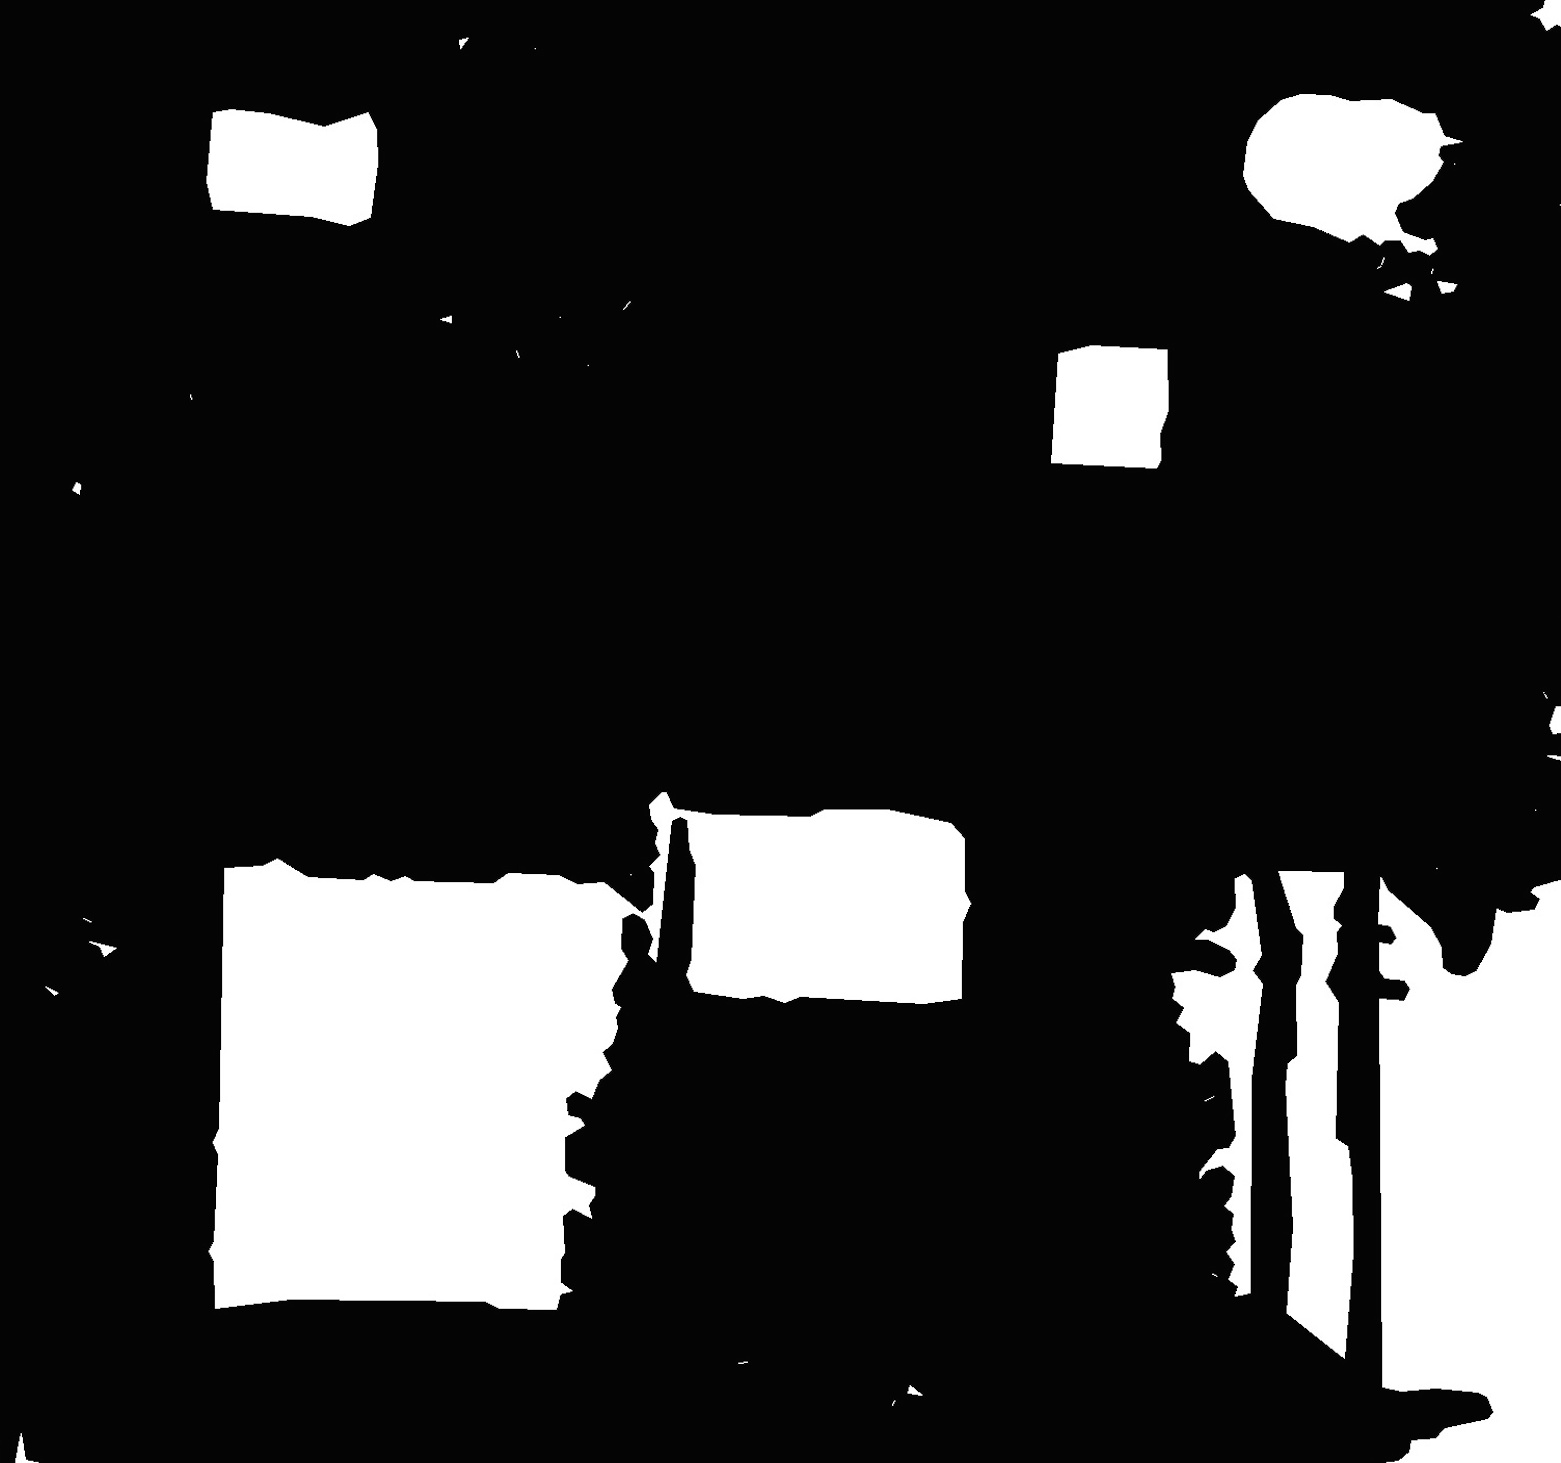
\includegraphics[width=\textwidth]{processed3}
                \caption{Time = $T_{N-2}$}
                \label{fig:third latest image}
        \end{subfigure}
        \caption{IMAGES AT THREE DIFFERENT TIMES}\label{fig:individual maps}
\end{figure}%
%

%\begin{figure}[t]
%\begin{center}
%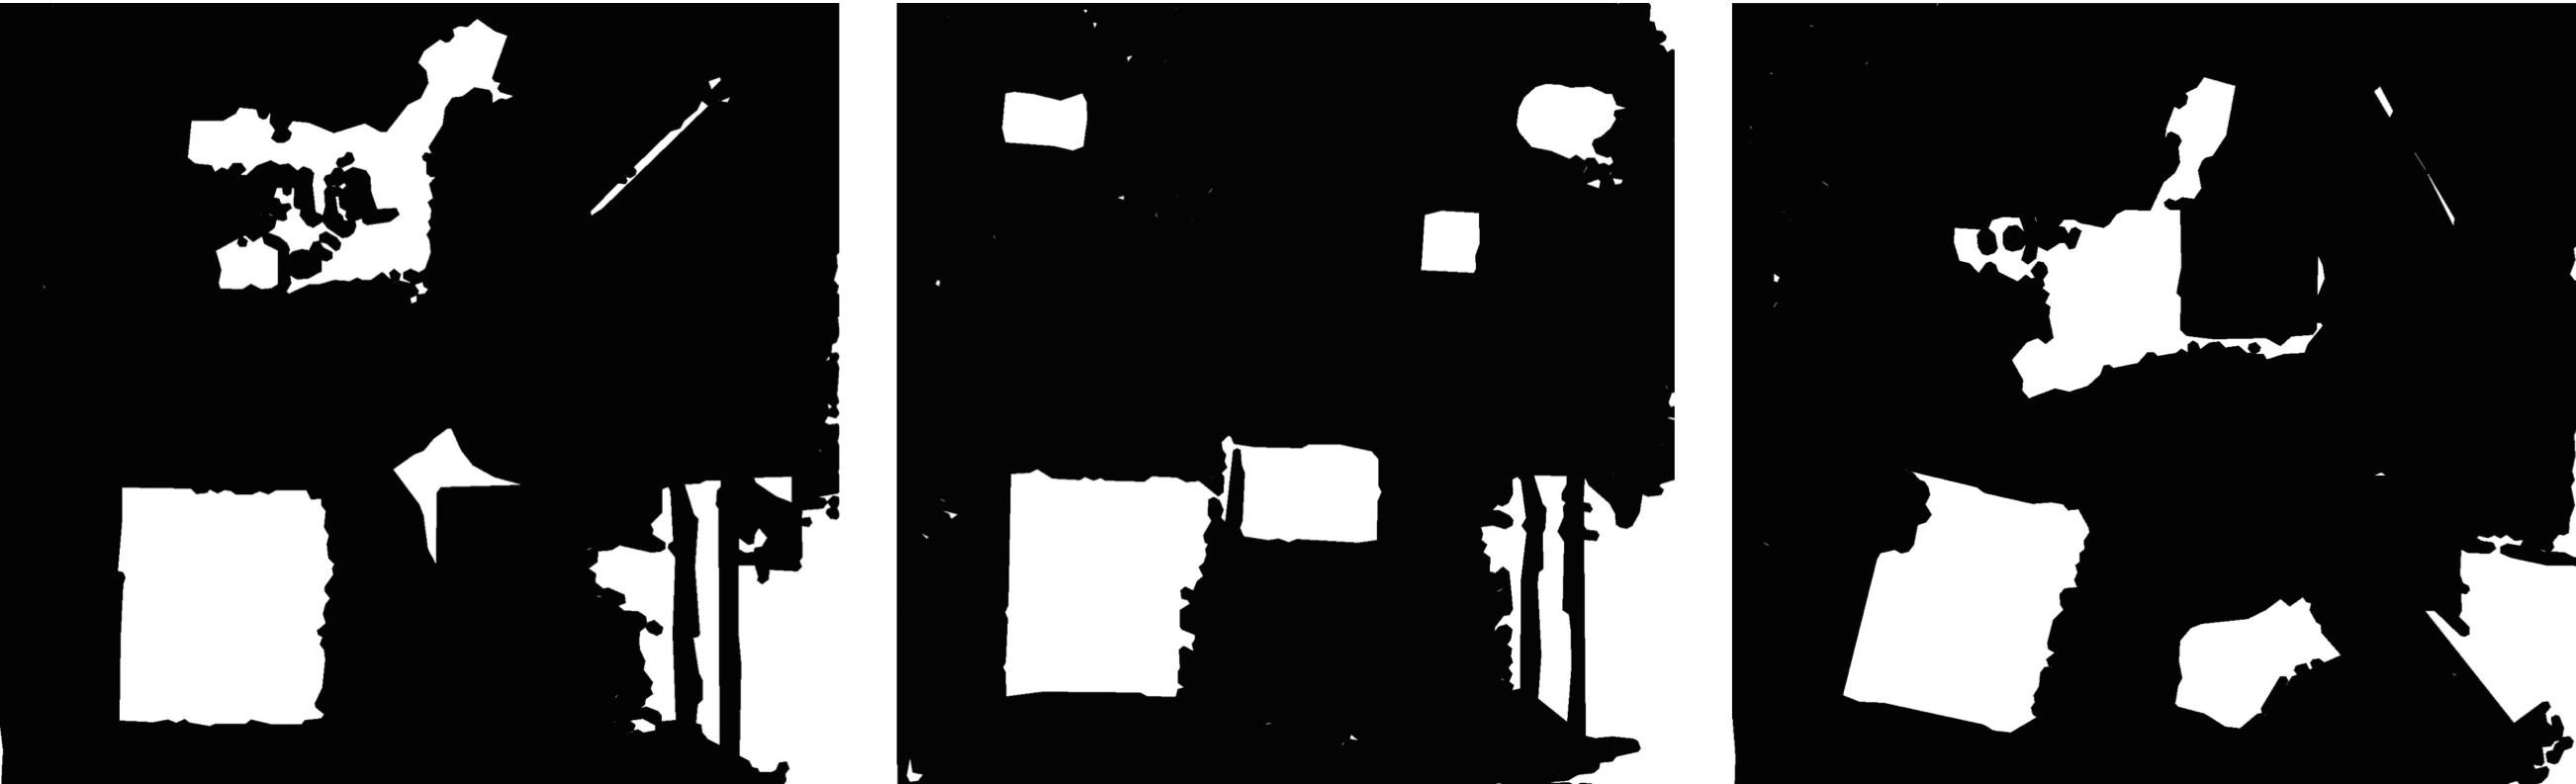
\includegraphics[width=3.5in]{processed_img}
%\caption{IMAGES AT THREE DIFFERENT TIMES}
%\label{default}
%\end{center}
%\end{figure}

\begin{figure}[t]
\begin{center}
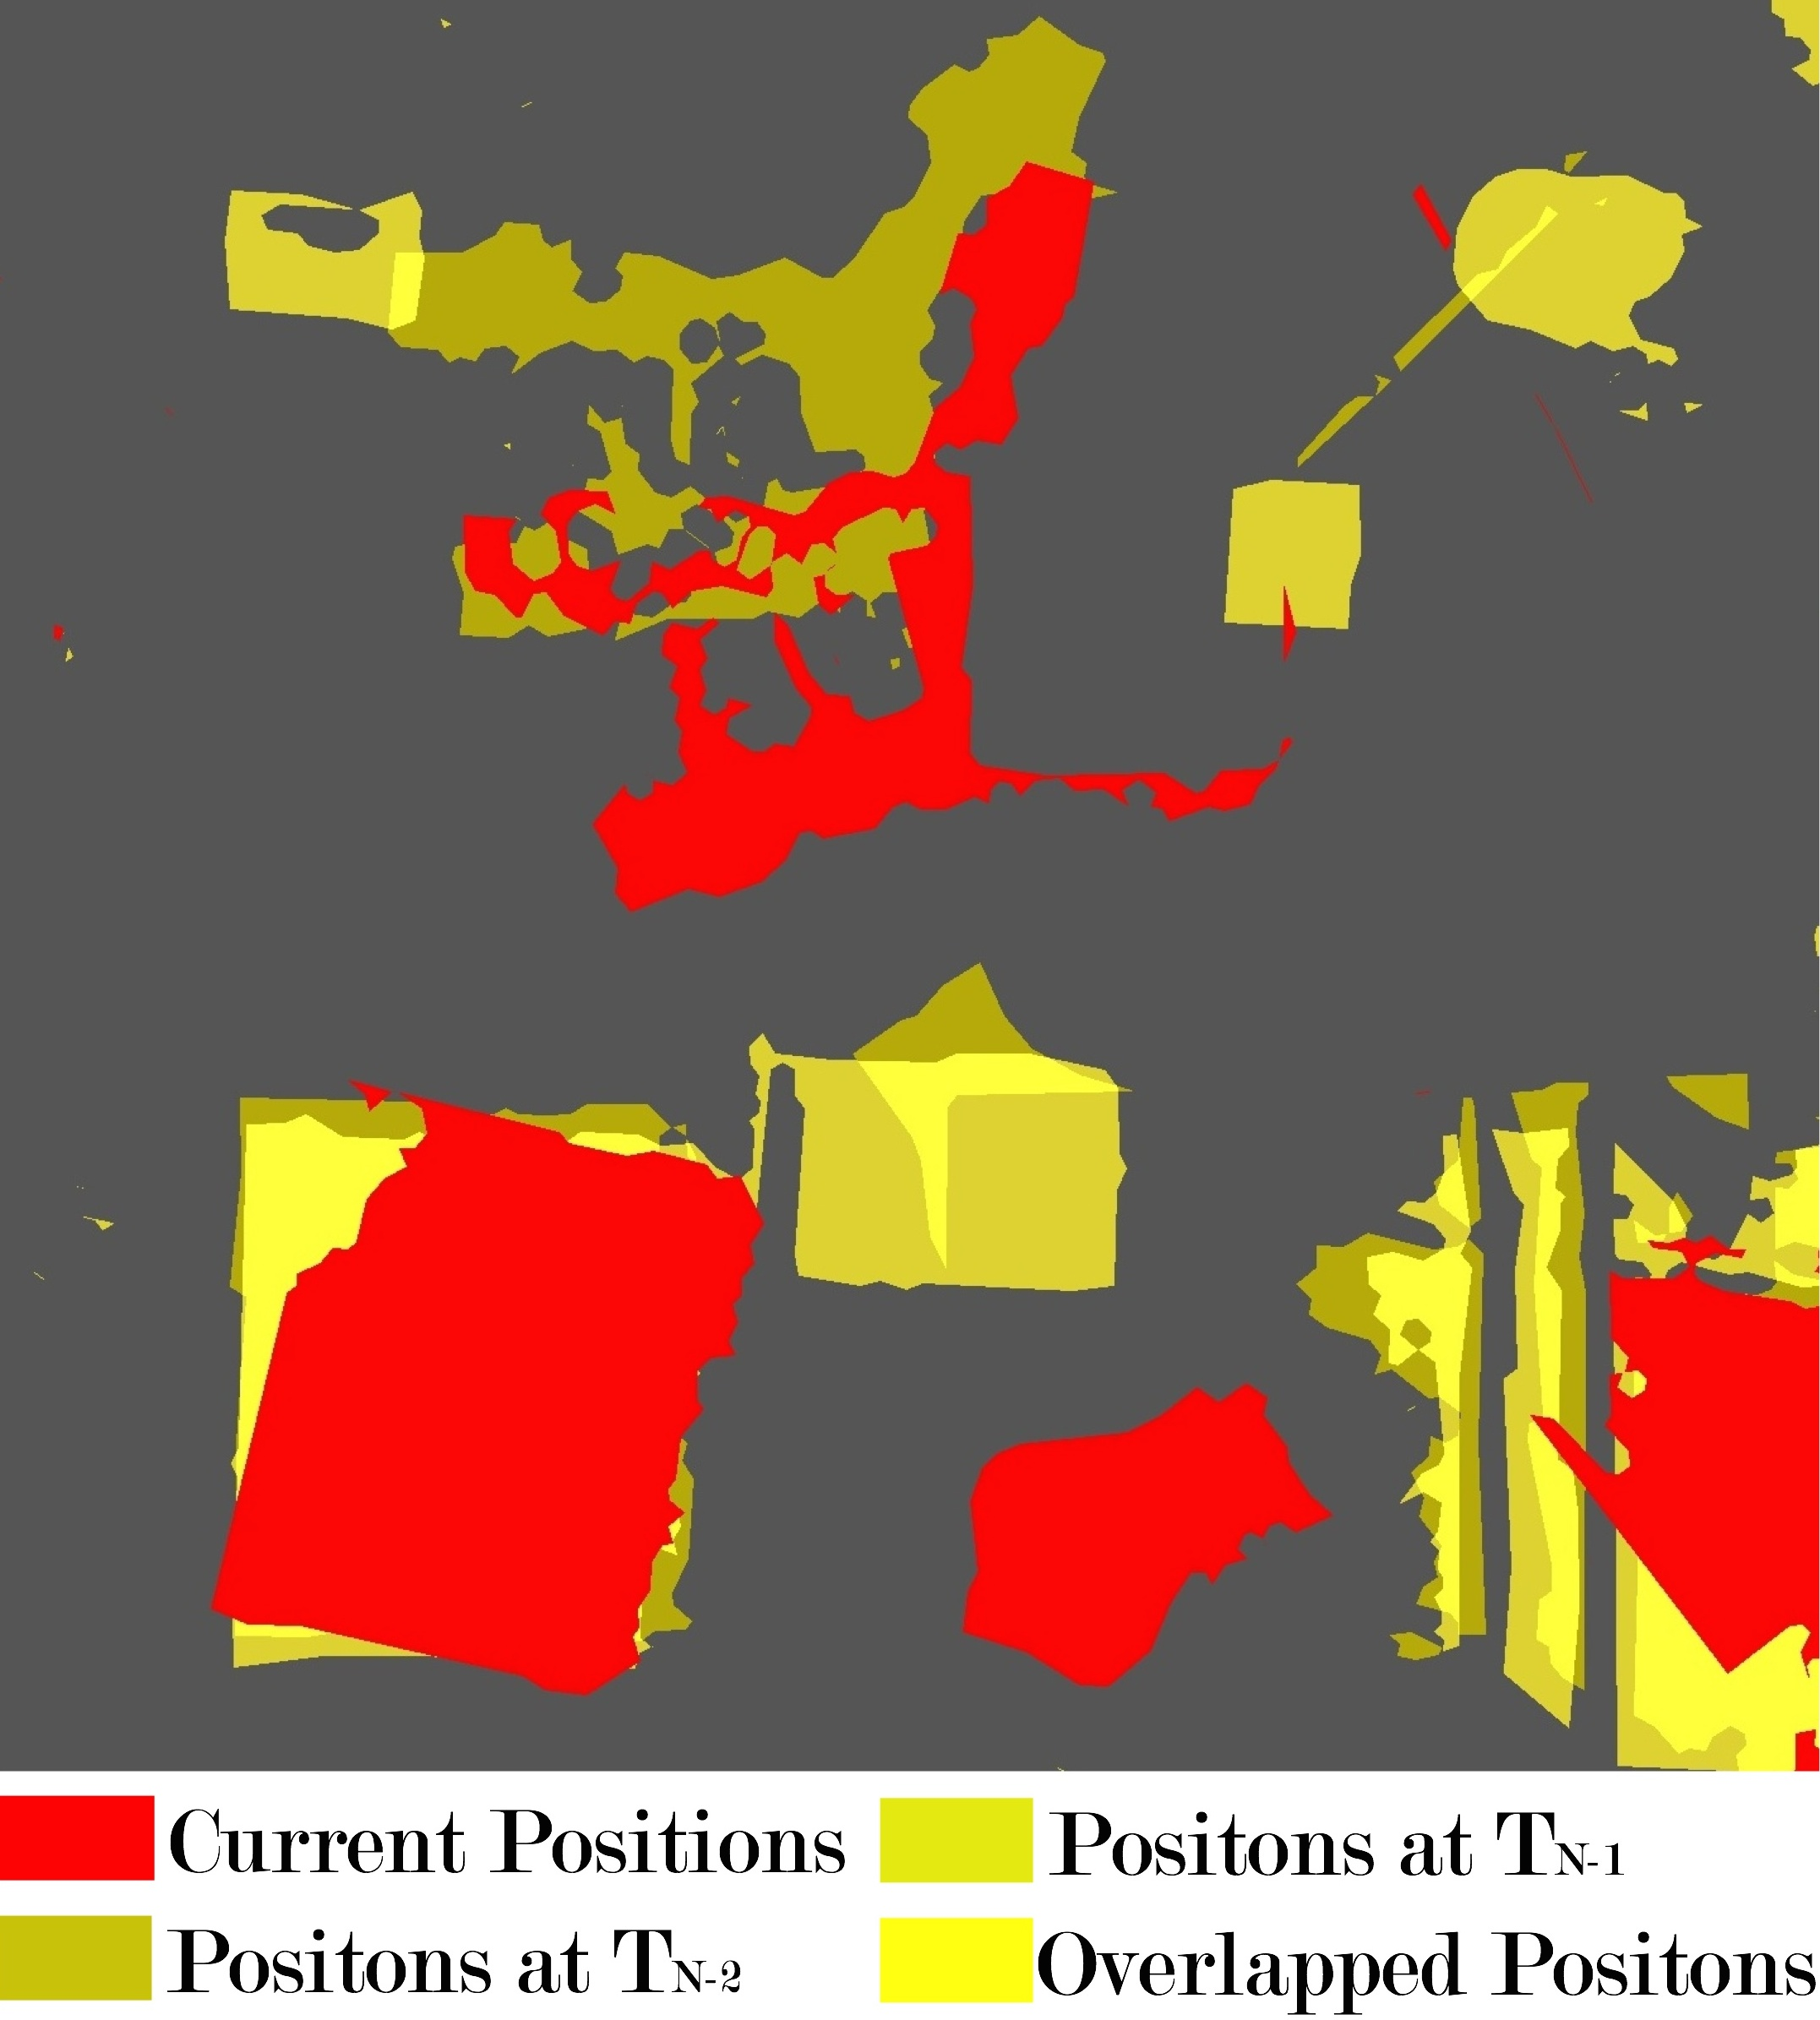
\includegraphics[width=3.5in]{overlapped}
\caption{FINAL WORKSPACE MAP}
\label{default}
\end{center}
\end{figure}

\section*{Analysis of Algorithm}
Although this mapping technique is very promising, there are some problems. The background detection method described is sensitive to noise and lighting. The thresholding is also sensitive. If there is an object which has the same color as the background, it will go undetected. If the background pixel has a wide range of values, the thresholding range has to be bigger, which means there will be a greater chance of missing obstacles. In addition, it is difficult to find the optimum value of the threshold range for a particular workspace. Depending on the time of the day, the lighting condition changes in the workspace, which makes adjustment necessary. 

\begin{figure}[t]
\begin{center}
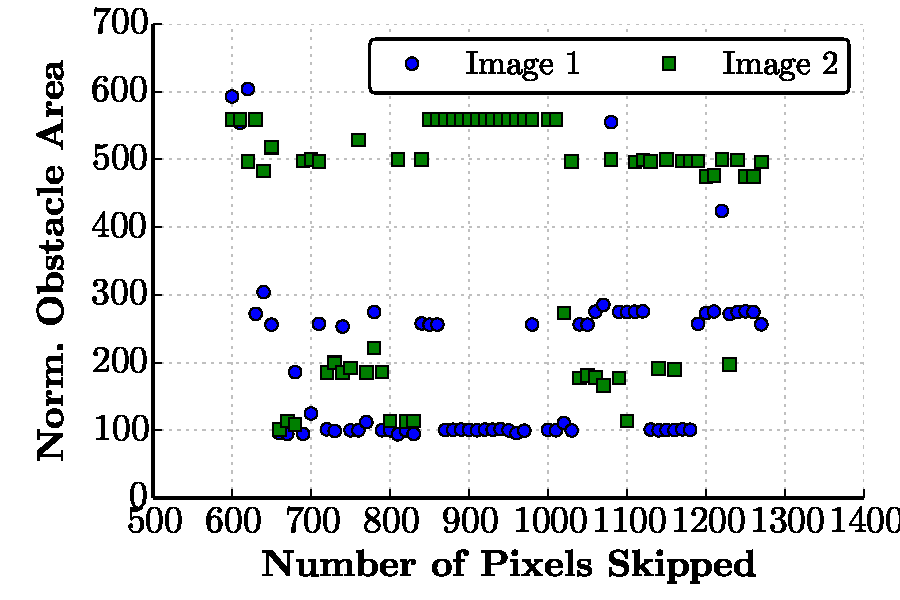
\includegraphics[width=3.5in]{SkippedPixels_v_ObstacleArea}
\caption{PERCENTAGE OF OBSTACLE DETECTED VERSUS NUMBER OF PIXEL SKIPPED}
\label{default}
\end{center}
\end{figure}

%
\begin{figure}[t]
\begin{center}
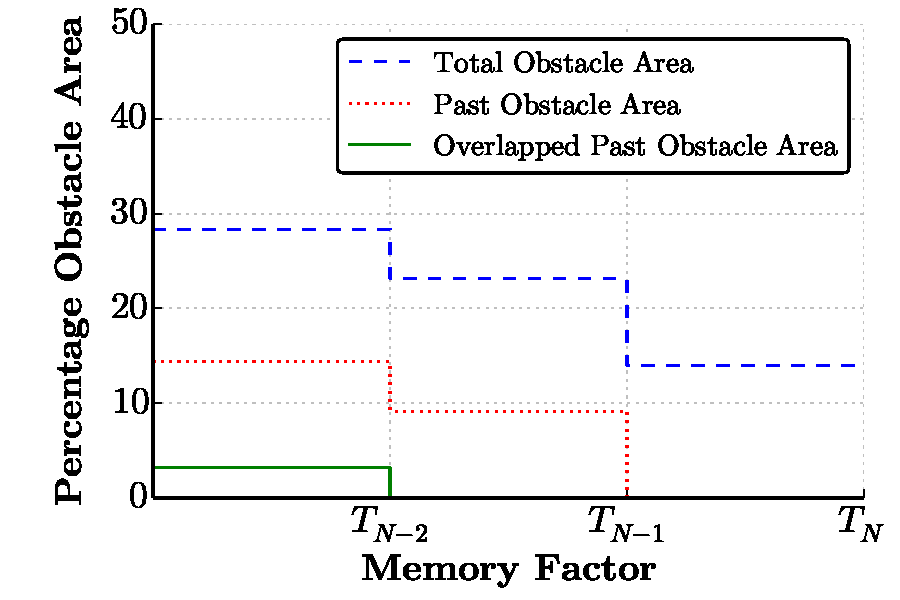
\includegraphics[width=3.5in]{area_vs_forgetting_factor}
\caption{OBSTACLE DETECTED AS A PERCENTAGE OF TOTAL WORKSPACE AREA VERSUS MEMORY FACTOR}
\label{default}
\end{center}
\end{figure}
%

The mapping performance depends on the accuracy of background detection. Figure 13 shows the effect of number of pixel skipped for background detection. The map which was most representative of the actual obstacles in the workspace was set as a benchmark. In Figure 13, the area of detected obstacles is shown as a percentage of the obstacle area detected in the benchmark map as a function of the number of pixels skipped. For first image, there are three ranges of number of pixel values skipped for which 100\% of the optimum obstacle area is detected. For second image, the range is reduced to two small ranges, which makes it difficult to find the optimum number of pixel skipped for 100\% obstacle detection. This is a major weakness of this algorithm.


Figure 14 shows the effect of memory factor on obstacle detected as a percentage of total workspace area. The total obstacle area, past obstacle areas and the overlap between past obstacle areas are shown. Obstacles occupy more area if the memory factor is bigger. In this example, when the memory factor is greater than $T_{N-2}$, all three individual maps are taken into account. The area occupied by obstacles is greater. When the memory factor is less than $T_{N-2}$ but greater than $T_{N-1}$, the oldest of the three individual maps is forgotten. In this case, both the total obstacle area and past obstacle area are smaller. If the memory factor is less than $T_{N-1}$, only the most recent individual map is taken into account, the other two are forgotten. The total obstacle area is the smallest in this case, and there is no past obstacle area shown in the map in yellow.
%The blind spot created by the payload may be dangerous if there is a obstacle right under it, which goes undetected.

%The mapping process can be improved to a 3D map, which takes the height of the obstacles into account. Disparity map using stereo vision might be a good way to do that. It will also solve some of the problems occurred in 2D mapping. Anything higher than the ground level can be assumed as an obstacle. The height-based object detection method can eliminate the drawbacks of color-based object detection. Combining these two techniques can be more robust than applying them individually.

\section*{Conclusion}
In this paper, a new approach of crane workspace mapping in near real-time using machine vision was presented. An algorithm for processing individual images and combining them into a complete map was shown. A technique to show areas where there were obstacles recently, along with current positions of the obstacles was also described. The effect of changing the design parameters, such as number of pixels skipped for obstacle detection and the choice of memory factor, on the mapping performance was also discussed. 
%\subsection*{Second-Level Heading}
%
%The next level of heading is boldface with upper and lower case letters. The heading is flushed left with the left margin. The spacing to the next heading is two line spaces.
%
%%%%%%%%%%%%%%%%%%%%%%%%%%%%%%%%%%%%%%%%%%%%%%%%%%%%%%%%%%%%%%%%%%%%%%%
%\subsubsection*{Third-Level Heading.}
%
%The third-level of heading follows the style of the second-level heading, but it is indented and followed by a period, a space, and the start of corresponding text.
%
%%%%%%%%%%%%%%%%%%%%%%%%%%%%%%%%%%%%%%%%%%%%%%%%%%%%%%%%%%%%%%%%%%%%%%%
%\section*{PAPER NUMBER}
%
%ASME assigns each accepted paper with a unique number. Replace {\bf DETC98/DAC-1234} in the input file preamble (the location will be obvious) with the paper number supplied to you  by ASME for your paper.


%%%%%%%%%%%%%%%%%%%%%%%%%%%%%%%%%%%%%%%%%%%%%%%%%%%%%%%%%%%%%%%%%%%%%%
%\section*{USE OF SI UNITS}
%
%An ASME paper should use SI units.  When preference is given to SI units, the U.S. customary units may be given in parentheses or omitted. When U.S. customary units are given preference, the SI equivalent {\em shall} be provided in parentheses or in a supplementary table. 
%%%%%%%%%%%%%%%%%%%%%%%%%%%%%%%%%%%%%%%%%%%%%%%%%%%%%%%%%%%%%%%%%%%%%%%
%\section*{MATHEMATICS}
%
%Equations should be numbered consecutively beginning with (1) to the end of the paper, including any appendices.  The number should be enclosed in parentheses and set flush right in the column on the same line as the equation.  An extra line of space should be left above and below a displayed equation or formula. \LaTeX\ can automatically keep track of equation numbers in the paper and format almost any equation imaginable. An example is shown in Eqn.~(\ref{eq_ASME}). The number of a referenced equation in the text should be preceded by Eqn.\ unless the reference starts a sentence in which case Eqn.\ should be expanded to Equation.
%
%\begin{equation}
%f(t) = \int_{0_+}^t F(t) dt + \frac{d g(t)}{d t}
%\label{eq_ASME}
%\end{equation}

%%%%%%%%%%%%%%%%%%%%%%%%%%%%%%%%%%%%%%%%%%%%%%%%%%%%%%%%%%%%%%%%%%%%%%
%\section*{FIGURES AND TABLES}
%
%All figures should be positioned at the top of the page where possible.  All figures should be numbered consecutively and captioned; the caption uses all capital letters, and centered under the figure as shown in Fig.~\ref{figure_ASME}. All text within the figure should be no smaller than 7~pt. There should be a minimum two line spaces between figures and text. The number of a referenced figure or table in the text should be preceded by Fig.\ or Tab.\ respectively unless the reference starts a sentence in which case Fig.\ or Tab.\ should be expanded to Figure or Table.
%
%
%%%%%%%%%%%%%%%%%%%%%%%%%%%%%%%%%%%%%%%%%%%%%%%%%%%%%%%%%%%%%%%%%%%%%%%
%%%%%%%%%%%%%%%%% begin figure %%%%%%%%%%%%%%%%%%%
%\begin{figure}[t]
%\begin{center}
%\setlength{\unitlength}{0.012500in}%
%\begin{picture}(115,35)(255,545)
%\thicklines
%\put(255,545){\framebox(115,35){}}
%\put(275,560){Beautiful Figure}
%\end{picture}
%\end{center}
%\caption{THE FIGURE CAPTION USES CAPITAL LETTERS.}
%\label{figure_ASME} 
%\end{figure}
%%%%%%%%%%%%%%%%% end figure %%%%%%%%%%%%%%%%%%% 
%%%%%%%%%%%%%%%%%%%%%%%%%%%%%%%%%%%%%%%%%%%%%%%%%%%%%%%%%%%%%%%%%%%%%%%
%
%
%
%
%%%%%%%%%%%%%%%%%%%%%%%%%%%%%%%%%%%%%%%%%%%%%%%%%%%%%%%%%%%%%%%%%%%%%%%
%%%%%%%%%%%%%%%% begin table   %%%%%%%%%%%%%%%%%%%%%%%%%%
%\begin{table}[t]
%\caption{THE TABLE CAPTION USES CAPITAL LETTERS, TOO.}
%\begin{center}
%\label{table_ASME}
%\begin{tabular}{c l l}
%& & \\ % put some space after the caption
%\hline
%Example & Time & Cost \\
%\hline
%1 & 12.5 & \$1,000 \\
%2 & 24 & \$2,000 \\
%\hline
%\end{tabular}
%\end{center}
%\end{table}
%%%%%%%%%%%%%%%%% end table %%%%%%%%%%%%%%%%%%% 
%%%%%%%%%%%%%%%%%%%%%%%%%%%%%%%%%%%%%%%%%%%%%%%%%%%%%%%%%%%%%%%%%%%%%%%
%
%All tables should be numbered consecutively and  captioned; the caption should use all capital letters, and centered above the table as shown in Table~\ref{table_ASME}. The body of the table should be no smaller than 7 pt.  There should be a minimum two line spaces between tables and text.

%%%%%%%%%%%%%%%%%%%%%%%%%%%%%%%%%%%%%%%%%%%%%%%%%%%%%%%%%%%%%%%%%%%%%%
%\section*{FOOTNOTES\protect\footnotemark}
%\footnotetext{Examine the input file, asme2e.tex, to see how a footnote is given in a head.}
%
%Footnotes are referenced with superscript numerals and are numbered consecutively from 1 to the end of the paper\footnote{Avoid footnotes if at all possible.}. Footnotes should appear at the bottom of the column in which they are referenced.


%%%%%%%%%%%%%%%%%%%%%%%%%%%%%%%%%%%%%%%%%%%%%%%%%%%%%%%%%%%%%%%%%%%%%%
%\section*{CITING REFERENCES}
%
%%%%%%%%%%%%%%%%%%%%%%%%%%%%%%%%%%%%%%%%%%%%%%%%%%%%%%%%%%%%%%%%%%%%%%%
%The ASME reference format is defined in the authors kit provided by the ASME.  The format is:
%
%\begin{quotation}
%{\em Text Citation}. Within the text, references should be cited in  numerical order according to their order of appearance.  The numbered reference citation should be enclosed in brackets.
%\end{quotation}
%
%The references must appear in the paper in the order that they were cited.  In addition, multiple citations (3 or more in the same brackets) must appear as a `` [1-3]''.  A complete definition of the ASME reference format can be found in the  ASME manual \cite{asmemanual}.
%
%The bibliography style required by the ASME is unsorted with entries appearing in the order in which the citations appear. If that were the only specification, the standard {\sc Bib}\TeX\ unsrt bibliography style could be used. Unfortunately, the bibliography style required by the ASME has additional requirements (last name followed by first name, periodical volume in boldface, periodical number inside parentheses, etc.) that are not part of the unsrt style. Therefore, to get ASME bibliography formatting, you must use the \verb+asmems4.bst+ bibliography style file with {\sc Bib}\TeX. This file is not part of the standard BibTeX distribution so you'll need to place the file someplace where LaTeX can find it (one possibility is in the same location as the file being typeset).
%
%With \LaTeX/{\sc Bib}\TeX, \LaTeX\ uses the citation format set by the class file and writes the citation information into the .aux file associated with the \LaTeX\ source. {\sc Bib}\TeX\ reads the .aux file and matches the citations to the entries in the bibliographic data base file specified in the \LaTeX\ source file by the \verb+\bibliography+ command. {\sc Bib}\TeX\ then writes the bibliography in accordance with the rules in the bibliography .bst style file to a .bbl file which \LaTeX\ merges with the source text.  A good description of the use of {\sc Bib}\TeX\ can be found in \cite{latex, goosens} (see how 2 references are handled?).  The following is an example of how three or more references \cite{latex, asmemanual,  goosens} show up using the \verb+asmems4.bst+ bibliography style file in conjunction with the \verb+asme2e.cls+ class file. Here are some more \cite{art, blt, ibk, icn, ips, mts, mis, pro, pts, trt, upd} which can be used to describe almost any sort of reference.

% Here's where you specify the bibliography style file.
% The full file name for the bibliography style file 
% used for an ASME paper is asmems4.bst.
\bibliographystyle{asmems4}


%%%%%%%%%%%%%%%%%%%%%%%%%%%%%%%%%%%%%%%%%%%%%%%%%%%%%%%%%%%%%%%%%%%%%%
%\begin{acknowledgment}
%Thanks go to D. E. Knuth and L. Lamport for developing the wonderful word processing software packages \TeX\ and \LaTeX. I also would like to thank Ken Sprott, Kirk van Katwyk, and Matt Campbell for fixing bugs in the ASME style file \verb+asme2e.cls+, and Geoff Shiflett for creating 
%ASME bibliography stype file \verb+asmems4.bst+.
%\end{acknowledgment}

%%%%%%%%%%%%%%%%%%%%%%%%%%%%%%%%%%%%%%%%%%%%%%%%%%%%%%%%%%%%%%%%%%%%%%
% The bibliography is stored in an external database file
% in the BibTeX format (file_name.bib).  The bibliography is
% created by the following command and it will appear in this
% position in the document. You may, of course, create your
% own bibliography by using thebibliography environment as in
%
% \begin{thebibliography}{12}
% ...
% \bibitem{itemreference} D. E. Knudsen.
% {\em 1966 World Bnus Almanac.}
% {Permafrost Press, Novosibirsk.}
% ...
% \end{thebibliography}

% Here's where you specify the bibliography database file.
% The full file name of the bibliography database for this
% article is asme2e.bib. The name for your database is up
% to you.
\bibliography{asme2e}
\begin{thebibliography}{9}

\bibitem{beavers}
J. E. Beavers, J. R. Moore, R. Rinehart and W. R. Schriver
``Crane-Related Fatalities in the Construction Industry,"
{\em Journal of Construction Engineering and Management,}
 Volume 132 Issue 9,September 2006.

\bibitem{cicb}
Crane Inspection and Certification Bureau, n.d., 
{\em from http://www.cicb.com/blog/posts/with-crane-related-injuries-on-the-rise-don-t-become-another-statistic.html}

\bibitem{Smith}
O. J. M. Smith,
``Feedback Control Systems,"
{\em New York: McGraw-Hill Book Co., Inc.},1958

\bibitem{Seering}
N. C. Singer and W. P. Seering,
``Preshaping command inputs to reduce system vibration,"
{\em Journal of Dynamic Systems, Measurement, and Control,}
Volume 112, pp. 76-82, March 1990.

%\bibitem{vaughan}
% J. Vaughan, A. Yano, and W. Singhose,
%``Robust negative input shapers for vibration suppression,"
% {\em Journal of Dynamic Systems, Measurement, and Control,}
%Volume 131, no. 3, p. 031014, 2009.
 
 \bibitem{w.sing}
 W. Singhose, N. Singer, and W. Seering,
 ``Time-optimal negative input shapers,"
 {\em J. of Dynamic Systems, Measurement, and Control,}
Volume 119, pp. 198-205, June 1997.
 
\bibitem{Singer}
N. Singer, W. Singhose, and E. Kriikku,
``An input shaping controller enabling cranes to move without sway,''
{\em ANS 7th Topical Meeting on Robotics and Remote Systems}, 
Volume 1, Augusta, GA, 1997, pp. 225-31. 

\bibitem{Sorensen}
K. Sorensen, W. Singhose, and S. Dickerson,
``A controller enabling
precise positioning and sway reduction in bridge and gantry cranes,"
{\em Control Engineering Practice,}
 Volume 15, no. 7, pp. 825-837, July 2007.

\bibitem{Khalid}
A. Khalid, W. Singhose, J. Huey, J. Lawrence and D. Frakes,
``Study of operator behavior, learning, and performance using an input-shaped bridge crane,"
{\em IEEE International Conference on Control Applications,}
 Volume 1, pp. 759-764, September 2004.
 
 \bibitem{Kim}
 D. Kim and W. Singhose,
``Performance studies of human operators driving double-pendulum bridge cranes"
{\em Control Engineering Practice,}
Volume 18, Issue 6, pp. 567-576, June 2010. 
 
\bibitem{changwan}
C. Kim, C. T. Haas,K. A. Liapi,and C. H. Caldas,
``Human-Assisted Obstacle Avoidance System Using 3D Workspace Modeling for Construction Equipment Operation,"
{\em journal of computing in civil engineering,}
Volume 20, Issue 3, pp. 177-186, May 2006.

\bibitem{murray}
D. Murray and C. Jennings,
``Stereo Vision Based Mapping and Navigation for Mobile Robots,"
{\em 1997 IEEE International Conference On Robotics And Automation,}
Volume 2, pp.1694-1699, April 1997.

\bibitem{felix}
F. Endres, J. Hess, J. Sturm, D. Cremers and W. Burgard,
``3-D Mapping With an RGB-D Camera,"
{\em IEEE Transactions on Robotics,}
volume 30, no.1, February 2014.

\bibitem{stiller}
C. Stiller, J. Hipp, C. Rossig, A. Ewald,
``Multisensor obstacle detection and tracking"
{\em Image and Vision Computing,}
Volume 18, Issue 5, pp. 389-396, April 2000.

\bibitem{klein}
G. Klein and D. Murray,
``Parallel Tracking and Mapping for Small AR Workspaces,"
{\em 6th IEEE and ACM International Symposium on Mixed and Augmented Reality,}
pp. 225-234, November 2007.

\bibitem{km}
G. Klein and D. Murray,
``Parallel Tracking and Mapping on a camera phone,"
{\em 8th IEEE International Symposium on Mixed and Augmented Reality,}
pp. 83-86, October 19-22, 2009.

\bibitem{sebastian}
``Simultaneous Localization and Mapping,"
S. Thrun and J.J Leonard,  2008,
{\em Springer Handbook of Robotics,}
Springer Berlin Heidelberg, Part E.

\bibitem{dissa}
M.W.M.G. Dissanayake, P. Newman, S. Clark,  H.F. Durrant-Whyte,  M. Csorba,
``A solution to the simultaneous localization and map building (SLAM) problem,"
{\em IEEE Transactions on Robotics and Automation,}
Volume 17, pp. 229-241, June 2001.

\bibitem{Aviad}
A. Shapira, Y. Rosenfeld and I. Mizrahi,
``Vision System for Tower Cranes,"
{\em Journal of Construction Engineering and Management,}
Volume 134, Issue 5 pp. 320-332, May 2008.

\bibitem{Yang}
J. Yang, P. Vela, J. Teizer and  Z. Shi,
``Vision-Based Tower Crane Tracking for Understanding Construction Activity."
{\em Journal of Computing in Civil Engineering,}
Volume 28, Issue 1, pp. 103-112, January 2014.

\bibitem{Yoshida:06}
Y. Yoshida and K. Tsuzuki,
``Visual Tracking and Control of a Moving Overhead Crane Load,"
{\em 9th IEEE International Workshop on Advanced Motion Control,}
pp. 630-635, 2006.

\end{thebibliography}

\end{document}

%%%%%%%%%%%%%%%%%%%%%%%%%%%%%%%%%%%%%%%%%%%%%%%%%%%%%%%%%%%%%%%%%%%%%%
%\appendix       %%% starting appendix
%\section*{Appendix A: Head of First Appendix}
%Avoid Appendices if possible.
%
%%%%%%%%%%%%%%%%%%%%%%%%%%%%%%%%%%%%%%%%%%%%%%%%%%%%%%%%%%%%%%%%%%%%%%%
%\section*{Appendix B: Head of Second Appendix}
%\subsection*{Subsection head in appendix}
%The equation counter is not reset in an appendix and the numbers will
%follow one continual sequence from the beginning of the article to the very end as shown in the following example.
%\begin{equation}
%a = b + c.
%\end{equation}
%
%\end{document}
